%%%%%%%%%%%%%%%%%%%%%%%%%%%%%%%%%%%%%%%%%%%%%%%%%%%%%%%%%%%%%%%%%%%%%%%%%%%%
%                                                                          %
%              (C) Copyright 2004  ...                                     %
%                      All Rights Reserved                                 %
%								  	   %
%%%%%%%%%%%%%%%%%%%%%%%%%%%%%%%%%%%%%%%%%%%%%%%%%%%%%%%%%%%%%%%%%%%%%%%%%%%%

\documentclass[11pt]{article}
\usepackage{graphicx}
\usepackage{makeidx}
\usepackage{psfig}

\makeindex

% define margins, etc
\topmargin	0.1in
\oddsidemargin	0in
\evensidemargin	0in
\textheight	8.80in
\textwidth	6.50in
\marginparsep	0.25cm
\headheight	0in
\headsep	0in
%\footskip	0.5in
%\footheight	0in%

% define macros
%%%%%%%%%%%%%%%%%%%%%%%%%%%%%%%%%%%%%%%%%%%%%%%%%%%%%%%%%%
%  Copyright (C) 2005 WanT group                         %
%  This file is distributed under the terms of the       %
%  GNU General Public License.                           %
%  See the file `License'  in the root directory of      %
%  the present distribution,                             %
%  or http://www.gnu.org/copyleft/gpl.txt                %
%%%%%%%%%%%%%%%%%%%%%%%%%%%%%%%%%%%%%%%%%%%%%%%%%%%%%%%%%%
%
% generally useful macros
%
\newcommand{\htmlimage}[1] {}
\newcommand{\REFAND} {\&}
\newcommand{\ETALNP}{\mbox{\it et al}}
\newcommand{\ETAL}{\mbox{\ETALNP{\it.}}}
\newcommand{\eqnref}[1] {\mbox{eq (\ref{#1})}}
\newcommand{\mycite}[2] {\cite{#2}}

%
% macros for math conventions in the theory description.
%
\newcommand{\cc}{{*}}
\newcommand{\br}{{\vec{r}}}
\newcommand{\bpsi}{{\vec{\psi}}}
\newcommand{\bphi}{{\vec{\phi}}}
\newcommand{\brho}{{\bar \rho}}
\newcommand{\bk}{{\vec{k}}}
\newcommand{\bR}{{\vec{R}}}
\newcommand{\bF}{{\vec{F}}}
\newcommand{\dpsi}{{\delta\psi}}
\newcommand{\ttvu}{{\bpsi^{(k+1)}}}
\newcommand{\tepsilon}{{\epsilon^{(k)}}}
\newcommand{\epsilonkj}{{\epsilon^{(k)}_j}}
\newcommand{\psij}{{\psi_j}}
\newcommand{\psii}{{\psi_i}}
\newcommand{\epsilonj}{{\epsilon_{j}}}
\newcommand{\psik}{{{\bpsi}^{(k)}}}
\newcommand{\psikj}{{{\bpsi}^{(k)}_j}}
\newcommand{\psikone}{{{\bpsi}^{(k)}_1}}
\newcommand{\psikN}{{{\bpsi}^{(k)}_N}}
\newcommand{\dpsik}{{{{\delta\bpsi}^{(k)}}}}
\newcommand{\dpsikj}{{{{\delta\bpsi}^{(k)}_j}}}
\newcommand{\dpsikone}{{{{\delta\bpsi}^{(k)}_1}}}
\newcommand{\dpsikN}{{{{\delta\bpsi}^{(k)}_N}}}
\newcommand{\rkj}{{{\br}^{(k)}_j}}
\newcommand{\Psik}{{\Psi^{(k)}}}
\newcommand{\Phik}{{\Phi^{(k)}}}

\newcommand{\WANT} {{\sc WanT}}
\newcommand{\WANTSUBTITLE}{{\sc an integrated approach to ab initio electronic
transport from maximally-localized Wannier functions}}
\newcommand{\WANTNAME} {an integrated approach to ab initio electronic transport
from maximally-localized Wannier functions}
%\newcommand{\WANTDATE} {\today}
\newcommand{\WANTDATE} {October 2005}
\newcommand{\UGAUTHORS} {
A. Ferretti, A. Calzolari, C.~Cavazzoni and M. Buongiorno
Nardelli}
\newcommand{\WANTVERSION} {2.0.0}
\newcommand{\WANTNOTES} {(Restricted Draft: Do Not Release or Cite)}
\newcommand{\WANTADDRESS} {\underline{pdac@pi.ingv.it}}
\newcommand{\WANTURL} {www.wannier-transport.org}
% title of PDAC paper
\newcommand{\WANTPAPER} {PDAC: A transient, multiphase flow code
for the 3D simulation of pyroclastic dispersal dynamics}


%
% macros for style conventions when describing the program.
%

% name of class or object in program
\newcommand{\OBJ}[1] {{\tt#1}}

% name of file
\newcommand{\FIL}[1] {{\it #1}}

% name of directory
\newcommand{\DIR}[1] {$<${\it #1}$>$}

% function arguments
\newcommand{\FA}[2] {{\rm{\bf#1}\ {\it#2}}}

% global function name
\newcommand{\FN}[3] {{\rm\bf#1}\ {\tt #2(}#3{\tt)}}

% class member function name
\newcommand{\FNO}[4] {{\rm\bf#2}\ \OBJ{#1::}{\tt#3(}#4{\tt)}}

% list item, for optional components, parameters, etc.
\newcommand{\TTLISTITEM}[1] {\item {\tt #1} \\}
\newcommand{\RMLISTITEM}[1] {\item {\rm #1} \\}
\newcommand{\BOLDLISTITEM}[1] {\item {\bf #1} \\}
\newcommand{\EMLISTITEM}[1] {\item {\em #1} \\}
\newcommand{\LISTITEM}[1] {\RMLISTITEM{#1}}

%
% other generally useful macros
%

\newcommand{\UGTITLE} {User's Guide}
\newcommand{\RMTITLE} {Reference Manual}
\newcommand{\UGDESC} {\noindent This {\em\UGTITLE\/} describes how to run and use the various
features of the integrated \WANT\ approach. This guide includes a
description of the capabilities of the program, how to use these
capabilities, the necessary input files and formats, and how to
run the program on both uniprocessor and parallel machines.}

\newcommand{\RMDESC} {
The \WANT\ (\PDACNAME)\ {\em\RMTITLE\/} is intended for the user
who wants to overview the model equations and the numerical
technique or for the programmer who wants to cooperate to the
\WANTC\ development. The manual describes how the model equations
are discretized and solved, provides the explicative list of all
variables used in the numerical code and gives a brief description
of the parallelization strategy, so that the advanced user can
optimize the code efficiency on several computational platforms.}

\newcommand{\PG}{\WANT\ {\it Programmer's Guide\/}}
\newcommand{\UG}{\WANT\ {\it User's Guide\/}}
\newcommand{\RM}{\WANT\ {\it Reference Manual\/}}
\newcommand{\prettypar}{

\smallskip

}

\newcommand{\eg}{{\it e.g.\/}}
\newcommand{\ie}{{\it i.e.\/}}

\newcommand{\KEY}[1]{{\tt #1}}
\newcommand{\IKEY}[1]{{\tt #1\index{#1 psfgen command}}}
\newcommand{\OKEY}[1]{$[${\tt #1}$]$}
\newcommand{\ARG}[1]{$<${\em #1}$>$}
\newcommand{\OARG}[1]{$[${\em #1}$]$}
\newcommand{\ARGDEF}[2]{$<${\em #1}$>$: #2}
\newcommand{\KEYDEF}[2]{{\tt #1}: #2}
\newcommand{\COMMAND}[4]{%
  #1 \\ {\bf Purpose:} #2 \\ {\bf Arguments:} #3 \\ {\bf Context:} #4 }

\newcommand{\icommand}[1]{#1\index{#1 command}}

\newcommand{\WANTCONF}[4]{%
%  \addcontentsline{toc}{subparagraph}{#1}%
  {\bf \tt #1 } $<$ #2 $>$ \\%
  \index{#1 parameter}
  {\bf Acceptable Values: } #3 \\%
  {\bf Description: } #4%
}

\newcommand{\WANTCONFWDEF}[5]{%
%  \addcontentsline{toc}{subparagraph}{#1}%
  {\bf \tt #1 } $<$ #2 $>$ \\%
  \index{#1 parameter}
  {\bf Acceptable Values: } #3 \\%
  {\bf Default Value: } #4 \\%
  {\bf Description: } #5%
}


\setcounter{secnumdepth}{3}
%% \setcounter{tocdepth}{5} %% very detailed table of contents
\setcounter{tocdepth}{4}

%
% the document itself
%

\begin{document}


% initial pages for the guide - title, TOC, etc.
%%%%%%%%%%%%%%%%%%%%%%%%%%%%%%%%%%%%%%%%%%%%%%%%%%%%%%%%%%%%%%%%%%%%%%%%%%%%

% title page

\thispagestyle{empty}

\vspace*{0.3in}

\begin{centering}
  \rule{6in}{0.04in}				\\	\vspace{0.25in}
  {\Huge \PDAC\ \UGTITLE}			\\	\vspace{0.25in}
  {\Large Version \PDACVERSION}          	\\	\vspace{0.20in}
  {\Large \PDACNOTES}                    	\\	\vspace{0.20in}
  \rule{6in}{0.04in}				\\	\vspace{0.25in}
  {\Large \UGAUTHORS}				\\	\vspace{0.20in}
  \PDACDATE					\\	\vspace{0.20in}
  \rule{6in}{0.04in}				\\	\vspace{0.25in}
  {\large       Istituto Nazionale di Geofisica e Vulcanologia} \\ 
  {\large       Pisa - Italy}      \\ 
\end{centering}
\vspace{0.2in}

\begin{center}
  {\Large \bf Description}
\end{center}

\noindent \UGDESC



% copyright and permissions notices
\newpage

\thispagestyle{empty}

\vspace*{0.1in}

\begin{centering}
{\LARGE \PDAC\ Version \PDACVERSION}\\
{\Large \PDACNOTES}\\
\bigskip
{\large Authors: \UGAUTHORS} \\
\medskip
{\large Istituto Nazionale di Geofisica e Vulcanologia } \\
\bigskip
{\large \copyright 2003 INGV.
All Rights Reserved} \\
\bigskip
\end{centering}

  \rule{6in}{0.04in}				\\	\vspace{0.25in}

\section*{PDAC (\PDACNAME )\\
Non-Exclusive, Non-Commercial Use License}

\subsubsection*{Introduction}

INGV, in cooperation wtih CNR and CINECA,
has developed the \PDACNAME\ \PDAC\
to the purpose of scientific research.
\PDAC\ is then available free of charge for
non-commercial use by individuals, academic or research institutions,
upon completion and submission of the online registration form available 
from the \PDAC\ web site \PDACURL.

Commercial use of the \PDAC\ software, or derivative works based thereon,
REQUIRES A COMMERCIAL LICENSE. Commercial use includes: 
(1) integration of all or part of the Software into a product for sale, 
lease or license by or on behalf of Licensee to third parties, or 
(2) distribution of the Software to third parties that need it to 
commercialize product sold or licensed by or on behalf of Licensee.  
INGV will negotiate commercial-use licenses for PDAC upon request. 
These requests can be directed to \PDACADDRESS

\subsubsection*{Registration}

Individuals may register in their own name or with their institutional or
corporate affiliations. Registration information must include name, title, 
and e-mail of a person with signature authority to authorize and commit the
individuals, academic or research institution, or corporation as necessary 
to the terms and conditions of the license agreement.

All parts of the information must be understood and agreed to as part of
completing the form. Completion of the form is required before software 
access is granted. Pay particular attention to the authorized requester 
requirements above, and be sure that the form submission is authorized 
by the duly responsible person.

Registration will be administered by the \PDAC\ development team.

\newpage
\subsubsection*{\PDAC: \PDACNAME\ LICENSE AGREEMENT}

Upon execution of this Agreement by the party identified below (``Licensee''),
The Istituto Nazionale di Geofisica e Vulcanologia (``INGV''), on 
behalf of the PDAC Development Team (``PDAC Team''),
will provide \PDAC\ in Executable 
Code and/or Source Code form (``Software'') to Licensee, subject to 
the following terms and conditions. For purposes of this Agreement, 
Executable Code is the compiled code, which is ready to run on Licensee's 
computer. Source code consists of a set of files which contain the 
actual program commands that are compiled to form the Executable Code.

1. The Software is intellectual property owned by INGV, and all 
right, title and interest, including copyright, remain with INGV. 
INGV grants, and Licensee hereby accepts, a restricted, non-exclusive, 
non-transferable license to use the Software for academic, research 
and internal business purposes only e.g. not for commercial use 
(see Paragraph 7 below), without a fee. Licensee agrees to reproduce 
the copyright notice and other proprietary markings on all copies of 
the Software. Licensee has no right to transfer or sublicense the 
Software to any unauthorized person or entity. However, Licensee does 
have the right to make complementary works that interoperate with PDAC, 
to freely distribute such complementary works, and to direct others 
to the PDAC Team's server to obtain copies of PDAC itself.

2. Licensee may, at its own expense, modify the Software to make derivative
works, for its own academic, research, and internal business purposes.
Licensee's distribution of any derivative work is also subject to the same
restrictions on distribution and use limitations that are specified herein
for INGV Software. Prior to any such distribution the Licensee shall 
require the recipient of the Licensee's derivative work to first execute a 
license for PDAC with INGV in accordance with the terms and conditions 
of this Agreement. Any derivative work should be clearly marked and 
renamed to notify users that it is a modified version and not the original 
PDAC code distributed by INGV.

3. Except as expressly set forth in this Agreement, THIS SOFTWARE IS 
PROVIDED ``AS IS'' AND INGV MAKES NO REPRESENTATIONS AND EXTENDS NO 
WARRANTIES OF ANY KIND, EITHER EXPRESS OR IMPLIED, INCLUDING BUT NOT 
LIMITED TO WARRANTIES OR MERCHANTABILITY OR FITNESS FOR A PARTICULAR 
PURPOSE, OR THAT THE USE OF THE SOFTWARE WILL NOT INFRINGE ANY PATENT, 
TRADEMARK, OR OTHER RIGHTS. LICENSEE ASSUMES THE ENTIRE RISK AS TO 
THE RESULTS AND PERFORMANCE OF THE SOFTWARE AND/OR ASSOCIATED MATERIALS. 
LICENSEE AGREES THAT INGV SHALL NOT BE HELD LIABLE FOR ANY DIRECT, 
INDIRECT, CONSEQUENTIAL, OR INCIDENTAL DAMAGES WITH RESPECT TO ANY 
CLAIM BY LICENSEE OR ANY THIRD PARTY ON ACCOUNT OF OR ARISING FROM 
THIS AGREEMENT OR USE OF THE SOFTWARE AND/OR ASSOCIATED MATERIALS.

4. Licensee understands the Software is proprietary to INGV. 
Licensee agrees to take all reasonable steps to insure that the Software 
is protected and secured from unauthorized disclosure, use, or release 
and will treat it with at least the same level of care as Licensee would 
use to protect and secure its own proprietary computer programs and/or 
information, but using no less than a reasonable standard of care. 
Licensee agrees to provide the Software only to any other person or 
entity who has registered with INGV. If licensee is not registering 
as an individual but as an institution or corporation each member of 
the institution or corporation who has access to or uses Software must 
understand and agree to the terms of this license. If Licensee becomes 
aware of any unauthorized licensing, copying or use of the Software, 
Licensee shall promptly notify INGV in writing. Licensee expressly 
agrees to use the Software only in the manner and for the specific uses 
authorized in this Agreement.

5. By using or copying this Software, Licensee agrees to abide by the
copyright law and all other applicable laws of Italy including, but 
not limited to, export control laws and the terms of this license. 
INGV shall have the right to terminate this license immediately by 
written notice upon Licensee's breach of, or non-compliance with, any 
of its terms. Licensee may be held legally responsible for any copyright 
infringement that is caused or encouraged by its failure to abide by 
the terms of this license. Upon termination, Licensee agrees to destroy 
all copies of the Software in its possession and to verify such 
destruction in writing.

6. The user agrees that any reports or published results obtained 
with the Software will acknowledge its use by the appropriate citation 
as follows: 

\begin{quote}
 PDAC was developed by the Volcanic Simulation Group,
 at the Istituto Nazionale di Geofisica e Vulcanologia - Italy.
\end{quote}

Any published work which utilizes PDAC shall include the following references: 

\begin{quote}
  Neri et al., ``Multiparticle simulation of collapsing volcanic columns 
  and pyroclastic flow'', {\em J.Geophys.Res}, vol.108, NO.B4 (2003)
\end{quote}

\begin{quote}
  Neri et al., ``\PDAC\ Reference Manual'' (2004)
\end{quote}

Electronic documents will include a direct link to the official PDAC page:

\begin{quote}
\PDACURL
\end{quote}

One copy of each publication or report will be supplied to INGV 
through Dr. Augusto Neri, at the addresses listed below in Contact 
Information.

7. Should Licensee wish to make commercial use of the Software, Licensee 
will contact INGV (\PDACADDRESS) to negotiate an appropriate 
license for such use. Commercial use includes: (1) integration of all 
or part of the Software into a product for sale, lease or license by or 
on behalf of Licensee to third parties, or (2) distribution of the 
Software to third parties that need it to commercialize product sold or 
licensed by or on behalf of Licensee.

8. Because substantial funds in the development of PDAC have been provided
by the European Commission, Gruppo Nazionale per la Vulcanologia (Italy)
and Ministero dell'Istruzione, dell'Universit\`a e della Ricerca (Italy),
any use, distribution or sublicense of the Software is subject to the specific
policies of these institutions.

9. PDAC is being distributed as a research and teaching tool and as such, 
the PDAC Team encourages contributions from users of the code that might, at 
INGV' sole discretion, be used or incorporated to make the basic 
operating framework of the Software a more stable, flexible, and
useful product. Licensees that wish to contribute their code to become 
an internal portion of the Software may be required to sign an 
``Agreement Regarding Contributory Code for PDAC Software''
before INGV can accept it (contact \PDACADDRESS\  for a copy).

\newpage
\subsubsection*{Contact Information}

The best contact path for licensing issues is by e-mail to \PDACADDRESS\ 
or send correspondence to:
\begin{verse}
                             PDAC Development Team\\
                             Istituto Nazionale di Geofisica e Vulcanologia\\
			     Centro di modellistica fisica e pericolosit\`a 
			     dei processi vulcanici\\
			     Sezione Sismologia e tettonofisica\\
                             32, Via della Faggiola\\
			     56126, Pisa - Italy\\
                             FAX: +39-0508311942
\end{verse}




% table of contents
\newpage
\tableofcontents

% list of figures
\newpage
\listoffigures

% list of tables
% \listoftables
%
% There are currently NO tables in either the User Guide or 
% the Programmer's Guide.  
%

\newpage


% Introduction
%%%%%%%%%%%%%%%%%%%%%%%%%%%%%%%%%%%%%%%%%%%%%%%%%%%%%%%%%%
%  Copyright (C) 2005 WanT group                         %
%  This file is distributed under the terms of the       %
%  GNU General Public License.                           %
%  See the file `License'  in the root directory of      %
%  the present distribution,                             %
%  or http://www.gnu.org/copyleft/gpl.txt                %
%%%%%%%%%%%%%%%%%%%%%%%%%%%%%%%%%%%%%%%%%%%%%%%%%%%%%%%%%%
\thispagestyle{empty}
\section{Theoretical Background}
\label{section:intro}

\noindent \WANT\ is an open-source, GNU General Public License
suite of codes that provides an integrated approach for the study
of coherent electronic transport in low-dimensional, extended
nanostructures. The core methodology combines state-of-the-art
Density Functional Theory (DFT), plane-waves, pseudopotential
calculations with a Green's functions method based on the Landauer
formalism to describe quantum conductance. The essential
connection between the two, and a crucial step in the calculation,
is the use of the maximally-localized Wannier function
representation to introduce naturally the ground-state electronic
structure into the lattice Green's function approach at the basis
of the evaluation of the quantum conductance. Moreover, the
knowledge of Wannier functions allows for a
direct link between the electronic transport properties of the
device with the nature of the chemical bonds, providing insight
into the mechanisms that govern electron flow at the nanoscale.
\\

\noindent \WANT\ scheme was originally described in Ref.~\cite{calz+04prb}:\\
A. Calzolari, N. Marzari, I. Souza, and M. Buongiorno Nardelli,\\
{\em Phys. Rev. B} {\bf 69}, 035108 (2004).
\\

\noindent In the following we review the theoretical background
that holds the \WANT\ method.


\subsection{Quantum transport}\label{subsec:tran}
%
Calculations of the quantum conductance are based on a
recently developed efficient method for evaluating quantum
transport in extended
systems~\cite{buon99prb,buon99prbr,buon+01prb}. This method is
applicable to any Hamiltonian that can be expanded within a
localized-orbital basis and can be used as a general theoretical
scheme for the computation and analysis of the electrical
properties of nanostructures.

\subsubsection{Electron transmission and Green's functions}
%
Let us consider a system composed of a conductor, $C$,
connected to two semi-infinite leads, $R$ and $L$, as in Fig.
\ref{fig:LCR}. A fundamental result in the theory of electronic
transport is that the zero-temperature conductance through a region of 
non-interacting
electrons (the $C$ region in Fig. \ref{fig:LCR}) is related to the
scattering properties of the region itself via the Landauer
formula~\cite{Landauer}:
%
%
\begin{equation}
{\mathcal C} = {2 e^2 \over h} {\mathcal T}(E_f),
\end{equation}
%
%
where ${\mathcal T}$ is the transmission function, ${\mathcal
C}$ is the conductance and $E_f$ the Fermi energy. 
The former represents the probability that
an electron injected at one end of the conductor will transmit to
the other end. In principle, we can compute the transmission
function for a coherent conductor\footnote{A conductor is said to
be coherent if it can be characterized by a transmission matrix
that relates each of the outgoing wave amplitudes to the incoming
wave amplitudes at a given energy.} starting from the knowledge of
the scattering matrix, $S$. The latter is the mathematical
quantity that describes the response at one lead due an excitation
at another. In principle, the scattering matrix can be uniquely
computed from the solution of the Schroedinger equation and would
suffice to describe the transport processes we are interested in
this work. However, it is a general result of conductance theory
that the elements of the S-matrix can be expressed in terms of the
Green's function of the conductor
\cite{datt95book,fish-lee81prb,meir-wing92prl} which, in practice,
can be sometimes simpler to compute.

Let us consider a physical system represented by an
Hamiltonian $H$. The Green's functions of the system can be
defined as: 
%
%
\begin{equation}
\label{eq:GF_def}
(\omega \pm i\eta-H) \, G(\omega)=I
\end{equation}
%
%
where $I$ is ht eidentity operator and 
$i\eta>0$ is an infinitesimal imaginary part added to the
energy to incorporate the boundary conditions into the equation.
The solution with $+$ sign is the retarded Green's function $G^r$,
while the solution with $-$ sign is called advanced Green's
function $G^a$. The transmission function can then be expressed in
terms of the Green's functions of the conductor and the couplings
of the conductor to the leads in a simple manner using the Fisher
and Lee formula~\cite{fish-lee81prb}:
%
%
\begin{equation}
{\mathcal T}(\omega) = {\rm Tr} \left[ 
            \Gamma_L G_C^r \Gamma_R G_C^a \right].
\label{eq:T}
\end{equation}
%
%
Here $G_C^{\{r,a\}}$ are the retarded and advanced
Green's functions of the conductor, and $\Gamma_{\{L,R\}}$ are
functions that describe the coupling of the conductor to the leads.

In the following we are going to restrict the discussion
to discrete systems that we can describe by ordinary matrix
algebra. More precisely, we are going to work with matrices
representing a physical system in the basis of localized
electronic orbitals centered on the atoms constituting the system.
It includes in particular the tight-binding model.
For a discrete media, the Green's function defined in Eq.~(\ref{eq:GF_def}) 
is then the inverse of the $(\omega - H)$ matrix.
To simplify the notation, we drop
the exponentis $\{a,r\}$ referring to advanced and retarded
functions and include the $\pm i\eta$ factor in $\omega$. For an open
system, consisting of a conductor and two semi-infinite leads (see
Fig. \ref{fig:LCR}), the above Green's function can be partitioned
into sub-matrices that correspond to the individual subsystems:
%
%
\begin{equation}
\left(
\begin{array}{lll}
g_L� & g_{LC} &� g_{LCR}\\
g_{CL} & G_C & g_{CR} \\
g_{LRC} & g_{RC} & g_R
\end{array}
\right) = \left(
\begin{array}{ccc}
\omega -h_L & -h_{LC} & 0\\
-h_{LC}^\dagger & \omega -H_C & -h_{CR}\\
0 & -h_{CR}^\dagger & \omega -h_R
\end{array}
\right)^{-1}, \label{condmatr}
\end{equation}
%
%
where the matrix $(\omega -H_C)$ represents the finite
``isolated'' conductor (with no coupling elements to the leads),
$(\omega -h_{\{R,L\}})$ represent the semi-infinite leads, and
$h_{CR}$ and $h_{LC}$ are the coupling matrices between the
conductor and the leads.
As a convention, we use lower case
letters for (semi-)infinite matrices and upper case for finite
dimension matrices. In Eq.~(\ref{condmatr}) we have made the
assumption that there is no direct interaction between the left
and right leads. From this equation it is straightforward to
obtain an explicit expression for $G_C$\cite{datt95book}:
%
%
\begin{equation}
   G_C(\omega) = (\omega -H_C -\Sigma_L(\omega) -\Sigma_R(\omega))^{-1} 
   \label{gconduct}
\end{equation}
%
%
where the finite dimension matrices
%
%
\begin{equation}
  \Sigma_L(\omega) = h_{LC}^\dagger (\omega -h_L)^{-1} h_{LC}, \;\;\;\;
  \Sigma_R(\omega) = h_{RC} (\omega -h_R)^{-1} h_{RC}^\dagger
\end{equation}
%
%
are defined as the self-energies due to the
semi-infinite leads. These terms can be viewed as
effective Hamiltonians that arise from the coupling of the
conductor with the leads. The coupling functions
$\Gamma_{\{L,R\}}(\omega)$ can then be obtained as~\cite{datt95book}:
%
%
\begin{equation}
   \Gamma_{\{L,R\}} = {\rm i} \left[ \Sigma_{\{L,R\}}^r(\omega) -
                      \Sigma_{\{L,R\}}^a(\omega) \right], 
   \label{eq:gamma}
\end{equation}
%
%
where the advanced self-energy $\Sigma_{\{L,R\}}^a$ is
the Hermitian conjugate of the retarded self-energy
$\Sigma_{\{L,R\}}^r$. The core of the problem lies in the
calculation of the self-energies of the semi-infinite leads.
%
%
\begin{figure}
   \begin{center}
     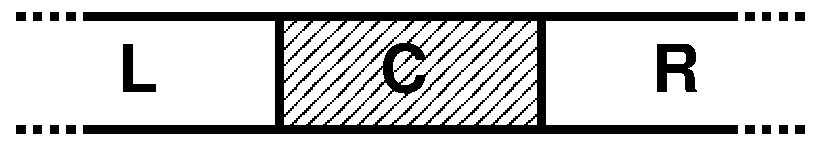
\includegraphics[width=0.45\textwidth]{fig1}
     \caption{A conductor described by the Hamiltonian $H_C$, connected
              to two semi-infinite leads $L$ and $R$, through the coupling
              matrices $h_{LC}$ and $h_{CR}$. \label{fig:LCR} }
   \end{center}
\end{figure}

It is well known that any solid (or surface) can be
viewed as an infinite (semi-infinite in the case of surfaces)
stack of principal layers with nearest-neighbor interactions
\cite{lee-joan81prb,lee-joan81prb1}. This corresponds to
transforming the original system into a linear chain of principal
layers. For a lead-conductor-lead system, the conductor can be
considered as one principal layer sandwiched between two
semi-infinite stacks of principal layers. The next sections
are devoted to the computation of the self-energies using the
principal layers approach.

%%%%%%%%%%%%%%%%%%%%%%%%%%%%%%%%%%%%%%%%%%%%%%%%%%%%%%%%%%%%%%%%%%%

\subsubsection{Transmission through a bulk system.} 
\label{ss:bulk}
%
Within the principal layer approach, the matrix elements
of Eq.~(\ref{eq:GF_def}) between layer orbitals yield a series of
matrix equations for the Green's functions:
%
%
\begin{eqnarray}
\label{serie}
    (\omega -H_{00}) G_{00} & = & I + H_{01}G_{10}\\
\nonumber
    (\omega -H_{00}) G_{10} & = & H_{01}^\dagger G_{00} + H_{01}G_{20}\\
\nonumber
                        \dots\\
\nonumber
    (\omega -H_{00}) G_{n0} & = & H_{01}^\dagger G_{n-1,0} +
                        H_{01}G_{n+1,0}
\end{eqnarray}
%
%
where the finite dimension matrices $H_{nm}$ and
$G_{nm}$ are formed by the matrix elements of the Hamiltonian and
Green's function between the layer orbitals. We assume that in a
bulk system $H_{00}=H_{11}=\dots$ and $H_{01}=H_{12}=\dots$.
Following Refs.~\cite{LopezSancho1,LopezSancho2}, this chain can be
transformed in order to express the Green's function of an
individual layer in terms of the Green's function of the preceding
(or following) one. This is done via the introduction of the
transfer matrices $T$ and $\overline{T}$, defined such that
$G_{10}=TG_{00}$
and $G_{00}=\overline{T}G_{10}$.
Using these definitions, we can write the bulk Green's
function as~\cite{Garcia2}:
%
%
\begin{equation}
    \label{eq:GT} G(\omega) = (\omega - H_{00} - H_{01}T
                  -H_{01}^\dagger \overline{T})^{-1}.
\end{equation}
%
%
The transfer matrix can be easily computed from the
Hamiltonian matrix elements via an iterative procedure, as
outlined in \cite{LopezSancho1,LopezSancho2}. In particular $T$
and $\overline T$ can be written as:
%
%
\begin{eqnarray}
   T &=& t_0 + \tilde{t}_0t_1 + \tilde{t}_0\tilde{t}_1t_2+\ldots+
   \tilde{t}_0\tilde{t}_1\tilde{t}_2\cdots t_n  \, ,\\
\nonumber
   \overline T &=& \tilde{t}_0 + t_0\tilde{t}_1 +t_0t_1\tilde{t}_2
   +\ldots+ t_0t_1t_2\cdots\tilde{t}_n \, ,
\end{eqnarray}
%
%
where $t_i$ and $\tilde{t}_i$ are defined via the recursion
formulas:
%
%
\begin{eqnarray}
   t_i &=& (I -t_{i-1}\tilde{t}_{i-1} - \tilde{t}_{i-1}t_{i-1})^{-1}
   t_{i-1}^2 , \\
   \tilde{t}_i &=& (I -t_{i-1}\tilde{t}_{i-1} -
   \tilde{t}_{i-1}t_{i-1})^{-1} \tilde{t}_{i-1}^2 ,
\nonumber
\end{eqnarray}
%
%
and
%
%
\begin{eqnarray}
   t_0 &=& (\omega - H_{00})^{-1} H_{01}^\dagger,\\
   \tilde{t}_0 &=& (\omega - H_{00})^{-1} H_{01}.
\nonumber
\end{eqnarray}
%
%
\noindent The process is repeated until $t_n,\tilde{t}_n \le
\delta$ with $\delta$ arbitrarily small. Usually, no more than 5 or
6 iterations are required to converge the above sum.

If we compare Eq.~(\ref{eq:GT}) with Eq.~(\ref{gconduct}), 
in the hypothesis of leads and conductors being
of the same material (bulk conductivity), we can identify one
principal layer of the bulk system with the conductor $C$, so that
$H_{00}\equiv H_C$. In particular, by comparing with
Eq.(\ref{gconduct}), we obtain the expression of the self-energies
of the conductor-leads system:
%
%
\begin{equation}
\Sigma_L = H_{01}^\dagger \overline T, \;\;\;\;\; \Sigma_R = H_{01} T.
\label{eq:sigmabulk}
\end{equation}
%
%
The coupling functions are then obtained~\cite{buon99prb} from the sole
knowledge of the transfer matrices and the coupling Hamiltonian
matrix elements: $\Gamma_L=-{\rm Im}(H_{01}^\dagger \overline T)$ and
$\Gamma_R=-{\rm Im}(H_{01} \overline T)$.

%%%%%%%%%%%%%%%%%%%%%%%%%%%%%%%%%%%%%%%%%%%%%%%%%%%%%%%%%%%%%%%%%%%%

\subsubsection{Transmission through a left lead-conductor-right lead
(LCR) system.} \label{ss:LCR}
%
The procedure outlined above can also be applied to the
case of electron transmission through one or more interfaces,
between different media. For the calculation of conductances in
realistic experimental geometry, the method can be expanded to the
general configuration of a Left-lead-Conductor-Right-lead (LCR)
systems --- as displayed in Fig~.\ref{fig:LCR}. To study this case
we make use of the Surface Green's Function Matching (SGFM)
theory, pioneered by~\cite{Garcia1,Garcia2}.

We have to compute the Green's function $G_I$, where the
subscript $I$ refers to the interface region composed of two
principal layers --- one in each media --- (L, C, R in our case).
Using the SGFM method, $G_I$ is calculated from the bulk Green's
function of the isolated systems,  and the coupling between the
two principal layers at the two sides of the interface. Via the
calculation of the transmitted and reflected amplitudes of an
elementary excitation that propagates from one medium to another,
it can be shown that the interface Green's function obeys the
following secular equation~\cite{Garcia2}:
%
%
\begin{eqnarray}
\nonumber G_{LCR}&=& \left(
\begin{array}{ccc}
G_{L} & G_{LC} & G_{LR}\\
G_{CL} & G_{C} & G_{CR}\\
G_{RL} & G_{RC} & G_{R}\\
\end{array}
\right) \\ &=& \left(
\begin{array}{ccc}
\omega -H^L_{00} - (H^L_{01})^\dagger \overline T & -H_{LC} & 0\\
-H_{CL} & \omega -H_{C} & -H_{CR}\\
0 & -H_{RC} & \omega -H^R_{00} - H^R_{01} T \\
\end{array}
\right)^{-1}. \label{secular1}
\end{eqnarray}
%
%
where $H_{nm}^{\{L,R\}}$ are the block matrices of the
Hamiltonian between the layer orbitals in the left and right leads
respectively, and $T_{\{L,R\}}$ and $\overline{T}_{\{L,R\}}$ are
the appropriate transfer matrices. The latter are easily computed
from the Hamiltonian matrix elements via the iterative procedure
already described in the bulk case (Sec.\ref{ss:bulk}).
Correspondingly, $H_{LC}$ and $H_{CR}$ are the coupling matrices
between the conductor and the leads principal layers in contact
with the conductor.
It is straightforward to obtain in the form of
Eq.(\ref{gconduct}), $G_C = (\omega -H_C -\Sigma_L
-\Sigma_R)^{-1}$, where $\Sigma_{L}$ and $\Sigma_R$ are the
self-energy terms due to the semi-infinite leads, and
identify~\cite{buon99prb}:
%
%
\begin{equation}
  \begin{array}{ccl}
  \Sigma_L(\omega) & = & H_{LC}^\dagger \, (\omega -H_{00}^L-(H_{01}^L)^\dagger
                   \overline T_L)^{-1} \, H_{LC},\\ 
  \Sigma_R(\omega) & = & H_{CR} \, (\omega
                  -H_{00}^R-H_{01}^R T_R)^{-1} \, H_{CR}^\dagger.
  \end{array}
\end{equation}
%
%
The transmission function in the LCR geometry can then
be derived from Eq.(\ref{eq:T}) and (\ref{eq:gamma}).
%
The knowledge of the conductor's Green's function $G_C$
gives also direct information on the electronic spectrum of the
system via the spectral density of states:
%
%
\begin{equation}
   N(\omega)= -\frac{1}{\pi} {\rm Im}[{\rm Tr}(G_C(\omega))].
\end{equation}
%
%
We have assumed a truly one-dimensional chain of
principal layers, which is physical only for systems like
nanotubes or quantum wires that have a definite
quasi-one-dimensional character. The extension to a truly
three-dimensional case is straightforward using Bloch functions in
the directions perpendicular to the transport axis. The introduction
of the principal layer concept implies that along the direction of
the layer expansion the system is described by an infinite set of
$k_\bot$ while $k_\|$ are still good quantum numbers for the
problem. The above procedure effectively reduces the
three-dimensional system to a set of non-interacting
linear-chains, one for each $k_\|$~\cite{lee-joan81prb,lee-joan81prb1}. 
We can then use the usual $k$-point summation techniques to evaluate the
quantum conductance: 
%
%
\begin{equation}
    T(\omega) = \sum_{k_\|} w_{k_\|}T_{k_\|}(\omega)
\end{equation}
%
%
where $w_{k_\|}$ are the relative weights of the different $k_\|$
in the irreducible wedge of the surface Brillouin 
zone~\cite{Baldereschi:1}.

%%%%%%%%%%%%%%%%%%%%%%%%%%%%%%%%%%%%%%%%%%%%%%%%%%%%%%%%%%%%%%%%%%%


\subsection {Maximally localized Wannier functions}\label{subsec:wannier}
%
\subsubsection{Definition of the problem}
%
Bloch orbitals cannot be used directly to evaluate
electronic transport with the method outlined in Sec.~\ref{subsec:tran}. 
As we have pointed out, quantum conductance
is computed starting from the knowledge of the lattice Green's
function, whose calculation relies on a localized orbital
representation. Bloch
orbitals, that are intrinsically delocalized, have to be
transformed into {\em localized} functions in order to construct
the sparse, short-ranged matrix elements of the Hamiltonian. The
core of our proposed methodology is to use m{\em
aximally-localized Wannier functions} (WFs) for the system
considered. These are the most natural choice for a set of
localized orbitals that still span the same Hilbert space of the
Hamiltonian eigenfunctions: they allow to bridge plane-wave
electronic structure and lattice Green's function calculations in
a coherent fashion.

A Wannier function $w_{n{\bf R}}({\bf r})$, labeled by
the Bravais lattice vector {\bf R}, is usually defined via a
unitary transformation of the Bloch functions $\psi_{n{\bf
k}}({\bf r})$ of the $n$th band:
%
%
\begin{equation}
w_{n{\bf R}}({\bf r})=\frac{V}{(2\pi)^3}\int_{BZ}\psi_{n{\bf k}}({\bf r})
e^{-i{\bf k}\cdot{\bf R}} d^3k,
\label{wf}
\end{equation}
%
%
where V is the volume of the unit cell and the
integration is performed over the entire Brillouin Zone. It is
easy to show that the WFs defined as above form an orthonormal
basis set, and that any two of them, for a given index $n$ and
different ${\bf R}$ and ${\bf R^\prime}$, are just translational
images of each other. Note that, as WFs are
(continuous) linear combinations of Bloch functions with different
energies, they do not represent stationary states, but still span
the original Hilbert space.

The {\em ab-initio} eigenstates are well-defined,
modulus an arbitrary ${\bf k}$-dependent phase factor; thus, the
definition above does not lead to a unique set of Wannier
functions~\cite{kohn,kohn1}, since the electronic structure
problem is invariant for the transformation $\psi_{n{\bf k}}
\rightarrow e^{\phi_n({\bf k})} \psi_{n{\bf k}} $. Besides this
freedom in the choice of phases $\phi_n({\bf k})$ for the Bloch
functions, there is a more comprehensive gauge freedom stemming
from the fact that the many-body wavefunction is actually a Slater
determinant: a unitary transformation between orbitals will not
change the manifold, and will not change the total energy and the
charge density of the system. In all generality, starting with a
set of ${\mathcal N}$ Bloch functions with periodic parts
$u_{n{\bf k}}$, we can constructs infinite sets of ${\mathcal N}$
WFs displaying different spatial characteristics:
%
%
\begin{equation}
    w_{n{\bf R}}({\bf r})=\frac{V}{(2\pi)^3}\int_{BZ}
    \left[ \sum_m U_{mn}^{({\bf k})}
    \psi_{m{\bf k}}({\bf r}) \right]
    e^{-i{\bf k}\cdot{\bf R}} d^3k.
    \label{eq:MLWF}
\end{equation}
%
%
The unitary matrices $U^{({\bf k})}$ include also the
gauge freedom on phase factors afore mentioned~\cite{nicola}. \\

\noindent The present \WANT\ method is based on a localization algorithm
that allows to transform a set of Bloch functions -- calculated by means
of {\it ab initio} approaches -- into a unique set of Maximally localized
Wannier functions, as proposed by Marzari and Vanderbilt
in 1997~\cite{nicola}. The formulation of this minimum-spread
criterion extends the concept of \emph{localized molecular
orbitals}, proposed by Boys~\cite{boys} for molecules, to the
solid-state case. However, its generality allows to deal with both
``extended'' (periodic and disordered) systems as well as with
``isolated'' clusters and molecules, in the limit of large
supercells.

\subsubsection{Localization procedure}
%
For our purposes, we need to transform the Bloch
eigenstates in WFs with the narrowest spatial
distribution. Following the procedure proposed by Marzari and
Vanderbilt~\cite{nicola}, we search the particular unitary
matrix $U_{mn}^{({\bf k})}$ that transform the Bloch eigenstates
in the WFs with the narrowest spatial distribution.

A measure of the spatial delocalization of WFs is given
by a {\em Spread Operator} $\Omega$, defined as the sum of the
second moments of all the Wannier functions in a reference cell:
%
%
\begin{equation}
    \Omega=\sum_n [\langle r^2 \rangle_n - \langle {\bf r}
    \rangle_n^2] , \label{omega}
\end{equation}
%
%
where the sum is over a selected  group of bands, and
%
%
\begin{eqnarray}
    \langle {\bf r} \rangle_n &=&\langle {\bf 0}n | {\bf r} | {\bf 0}n \rangle, \\
    \nonumber
    \langle r^2 \rangle_n &=& \langle {\bf 0}n | r^2 | {\bf 0}n \rangle .
    \label{position}
\end{eqnarray}
%
%
The value of the spread $\Omega$ depends on the choice
of unitary matrices $U^{({\bf k})}$; thus  it is possible to
evolve any arbitrary set of $U^{({\bf k})}$ until we reach the stationarity
condition:
%
%
\begin{equation}
   \frac {\delta \Omega_{\bf k}}{\delta U^{({\bf k})}}=0
   \label{minimo}
\end{equation}
%
%
At the minimum, we obtain the matrices
$U^{({\bf k}), ML}$ that transform the first-principles
$\psi_{n{\bf k}}^{FP}({\bf r})$ into the {\em maximally-localized
WFs}, according to Eq.~(\ref{eq:MLWF}).
If we restrict to the case of {\bf k}-point mesh
calculations, we can use finite differences in reciprocal space to
evaluate the derivatives of Eq.~(\ref{minimo}). For this purpose we
rewrite the expectation values $\langle \mathbf{r} \rangle$ and 
$\langle r^2 \rangle $ as proposed by Blount~\cite{blount}:
%
%
\begin{eqnarray}
\label{eq:pos_k}
\langle {\bf 0}n | {\bf r} | {\bf 0}n  \rangle &=& i \frac{1}{N}
\sum_{ {\bf k} } e^{ +i{\bf k}\cdot{\bf R} } \langle u_{ {\bf k}n
}| \nabla_{\bf k} | u_{ {\bf k}n },  \rangle\\
%
\nonumber
\langle {\bf 0}n | r^2 | {\bf 0}n \rangle\ &=& \frac{1}{N} \sum_{
{\bf k}} e^{+i{\bf k}\cdot{\bf R}} \langle u_{ {\bf k}n }|
\nabla^2_{\bf k} | u_{ {\bf k}n }  \rangle, 
\end{eqnarray}
%
%
where $| u_{ n{\bf k} }  \rangle = e^{-i{\bf k}\cdot{\bf
r}} | \psi_{ n{\bf k} }  \rangle$ is the periodic part of the Bloch
function. Making the assumption that the BZ has been discretized
into a uniform {\bf k}-point mesh, and letting $ \mathbf{b} $ being 
the vectors
that connect a mesh point to its near neighbors, we can define the
overlap matrix between Bloch orbitals as:
%
%
\begin{equation}
   \label{overlap}
   M^{ ( \mathbf{k},\mathbf{b}) }_{ mn } = \langle u_{ m\mathbf{k} }| 
        u_{ n\mathbf{k}+\mathbf{b} }  \rangle = 
        \langle \psi_{ m \mathbf{k} } | e^{-i\mathbf{k}\mathbf{b}} | 
        \psi_{ n \mathbf{k}+\mathbf{b}} \rangle .
\end{equation}
%
%
Using the expression of the gradient  in terms of finite
differences and substituting $M^{ ({\bf k}, {\bf b})}_{ mn }$ in
Eq.~(\ref{eq:pos_k}) we obtain the expressions for $\langle \mathbf{r} \rangle$
and $\langle r^2 \rangle $
to be used in the localization procedure:
%
%
\begin{eqnarray}
\label{position2}
   \langle \mathbf{r} \rangle_{n} &=& -\frac{1}{N}
          \sum_{ \mathbf{k},\mathbf{b} } 
           w_b \, \mathbf{b} \, \text{Im} 
          \, \text{Ln} M^{ ({\bf k}, {\bf b})}_{ nn } \\ \nonumber
   \langle r^2 \rangle_n &=&  \frac{1}{N} \sum_{ {\bf k,b} } w_b
   \left[ \left( 1- |M^{ ({\bf k}, {\bf b}}_{ nn }|^2 \right) +
          \left( \text{Im}\, \text{Ln} M^{ ({\bf k}, {\bf b})}_{ nn } \right)^2 
   \right]
\end{eqnarray}
%
%
Here, $w_b$ are the weights of the $\mathbf{b}$-vectors, and
must satisfy the completeness condition $\sum_{\mathbf{b}} w_b
b_{\alpha}b_{\beta}= \delta_{{\alpha}{\beta}}$. Substituting the
above expression into Eq.~(\ref{omega}), we obtain the expression
for the spread operator as a function of the overlap matrix $M^{
({\bf k}, {\bf b})}_{ mn }$.

In order to calculate the gradient in Eq.~(\ref{minimo}),
we consider the first order change in $\Omega$ arising from an
infinitesimal transformation $U_{mn}^{({\bf k})} = \delta_{mn} +
dW_{mn}^{({\bf k})}$, where $dW$ is an infinitesimal antiunitary
matrix ($dW^{\dag} = - dW$). The gauge transformation rotates the
wave functions according to Eq.~(\ref{eq:MLWF}) into $| u_{ {\bf k}n }
\rangle \to | u_{ {\bf k}n } \rangle + \sum_mdW_{mn}^{({\bf k})}|
u_{ {\bf k}m } \rangle $. Following the elegant description of
Ref. \cite{nicola}, we obtain the final expression for the
gradient of the spread functional:
%
%
\begin{equation}
   \label{grad_fin}
   G^{({\bf k})}=\frac{\delta \Omega}{dW^{({\bf k})}}= 4 \sum_{ {\bf
   b} } w_b \left( \frac {R^{{\bf k,b})} -R^{({\bf
   k,b}) \, \dagger}}{2} - \frac {T^{({\bf k,b})}+T^{({\bf
   k,b}) \, \dagger}}{2i} \right)  
\end{equation}
%
%
where
%
%
\begin{equation}
   R_{mn}^{ ({\bf k,b}) } = M_{mn}^{ ({\bf k,b}) } M_{nn}^{ ({\bf
   k,b})\ast} ;\qquad T_{mn}^{ ({\bf k,b}) }= \frac{ M_{mn}^{ ({\bf
   k,b}) } } { M_{nn}^{ ({\bf k,b}) } } \left[ \text{Im}\, \text{Ln} M_{nn}^{({\bf
   k,b})} + {\bf b}\cdot \langle {\bf r} \rangle_n \right].
\end{equation}
%
%
Note that the entire expression $G^{({\bf k})}$ is a
function of the overlap matrices $M^{ ({\bf k,b}) }$.  The
minimization of the spread functional $\Omega$ is obtained via
steepest descent or conjugate gradient schemes.
The procedure does not require the updating of wavefunctions, but only
of the overlap and unitary matrixes. This is the most demanding task 
(scaling as $N^3$) for each iteration in Wannier localization.

Wannier functions obtained with the above procedure
should be almost real, except for an overall phase factor. 
This conjecture can also be used as a check of the convergence of the
localization procedure.
It is important to
notice that whenever a Born-von Karman discretization of the
Brillouin Zone is introduced, even the above-mentioned WFs are not
truly localized, but will be periodic in real-space, with a {\em
superperiodicity} determined by the BZ discretization. The truly
isolated limit is recovered only in the case of continuous BZ
integrations. This is easily seen remembering that $ \psi_{n{\bf
k}}({\bf r})= u_{n{\bf k}}({\bf r}) e^{i{\bf k}\cdot{\bf r}} $,
and $� u_{n{\bf k}}({\bf r}) $ has the periodicity of the direct
lattice; thus the phase factors $ e^{i{\bf k}\cdot{\bf r}}� $
determine the {\em superperiodicity} of the $ \psi_{n{\bf k}} $
themselves.

In the standard language of electronic-structure
calculations, if the $ \psi_{n{\bf k}} $ have ${\bf k}$'s that are
restricted to a uniform Monkhorst-Pack mesh, they will all be
periodic with a wavelength inversely proportional to the spacing
of the mesh; this periodicity is consequently inherited by the
WFs. For $\mathcal N$ {\bf k}-points along a direction of the BZ,
the WFs will repeat along the corresponding direction every
$\mathcal N$ cells. A dense mesh of {\bf k}-points guarantees that
the adjacent replicas of a WF are sufficiently far and do not
interact. However, even the case of $\Gamma$-sampling is
encompassed by the above formulation. In this case the neighboring
{\bf k}-points for $\Gamma$ are given by the homologous
$\Gamma$-points of the neighboring cells. In this case the algebra
becomes simpler and an equivalent real-space formulation is
preferred \cite{Silvestrelli,gammaUS}.

The method described above works properly in the case of
{\em isolated groups} of bands. A Bloch band is called {\em
isolated} if it does not become degenerate with any other band
anywhere in the BZ. Conversely, a group of bands is said to form a
{\em composite group} if bands are inter-connected by degeneracy,
but are {\em isolated} from all the other bands~\cite{nicola}. On
the other hand to study quantum conductance in extended systems we
often need to compute WFs for a subset of energy bands that are
entangled or mixed with other bands. Most often we are interested
in the states that lie in the vicinity of the Fermi level of a
conductor in a restricted energy range. Since the unitary
transformations $U^{({\bf k})}$ mix energy bands at each {\bf
k}-point, any arbitrary choice of states inside a prescribed
window will affect the localization properties of WFs unless
energy gaps effectively separate the manifold of interest from
higher and lower bands.
%
This problem has been solved by Souza, Marzari, and
Vanderbilt~\cite{ivo2}, introducing an additional disentanglement
procedure that automatically extracts the best
possible manifold of a given dimension from the states falling in
a predefined energy window. This is the generalization to {\em
entangled} or metallic cases of the maximally-localized WF
formulation. The procedure relies on minimizing the subspace
dispersion across the Brillouin Zone, and effectively extracts the
bands of interest from the overall band structure.

In practice, first we select a desired number of bands
in an energy window; then we determine the optimally-connected
subspace that can be extracted from that band structure; and
finally proceed with a standard localization procedure inside
the selected subspace. 
The resulting orbitals have the same good localization properties, and
allow to apply our formalism to arbitrary systems, independently
of the insulating or metallic nature of the band manifold. It
should be stressed that the WFs obtained in the later case are not
the WFs of the occupied subspace (that would exhibit poor
localization properties), but are those of a well connected,
continuous subspace that in general will contain both occupied and
unoccupied Bloch functions.

%%%%%%%%%%%%%%%%%%%%%%%%%%%%%%%%%%%%%%%%%%%%%%%%%%%%%
\subsubsection{Conditioned localization and penalty functionals}
\label{subsubsec:penalty}
The above described formalism adopts a localization criterion which is 
somehow {\it global}: the functional we want to minimize is the total spread, 
while we are often interested in the localization of 
each Wannier function in the selected set.
In this scenario it may happen that, in order to gain 
localization in the total spread one or more WFs may move their centers out of the
system ({\it e.g.} in the vacuum) and therefore make the remaining functions 
lleave to better localize. In this cases the final WF set is useless from our point of
view.

We therefore introduce the idea of {\it conditioned} localization adding some 
further {\it penalty} functional to the total spread. 
These penalty functionals may be use to drive the Wannier localization towards the
achievement of some required feature.
It maybe interesting {\it e.g.} to fix the problem of WFs moving in the vacuum region
to add a {\it spring} potential driving the functions to have their centers 
as close as possible to the positions we like. The form of the penalty functional 
is therefore:
%
%
\begin{equation}
\label{eq:penalty}
   \Omega_P = A \, \sum_{n} \, w_n\, \left[ \, \langle \mathbf{r} \rangle_n 
                            - \mathbf{r}_{n0} \, \right]^2 ,
\end{equation}
%
%
where $A$ is the functional amplitude, $w_n$ a weight, and $\mathbf{r}_{n0}$ 
is the chosen target position for the $n-$th WF. 
After some tedious algebra it is possible to write and explicit form for the 
derivative of this functional wrt $U^{(\mathbf{k})}$. This is then used to compute
the penalty contribution to the gradient during the minimization of the functional.
Setting to zero some weights $w_n$ we are also able to selectively switch off the 
conditioning on some WFs. 
Obviously many different kinds of such penalty functionals may be written.
We note that this procedure does not alter physical quantities such as the 
polarization, which is infact independent of the particular unitary rotations chosen
for the localization. 
The conditioned minimization fo Eq.~(\ref{eq:penalty}) is implemented in \WANT; 
see Sec.~\ref{sec:input} for more details about how to setup the input file.

%%%%%%%%%%%%%%%%%%%%%%%%%%%%%%%%%%%%%%%%%%%%%%%%%%%%%
\subsubsection{Real space hamiltonians}
%
In order to calculate the conductance according to the
prescriptions outlined in Sec.~\ref{subsec:tran}, we need as an input
the matrix elements of the Hamiltonian calculated on a localized
basis: in our case, it is the minimal basis of the
maximally-localized WFs. 
Assuming a BZ
sampling fine enough to eliminate the interaction with the
WF periodic images, we can simply compute the WF Hamiltonians 
$H_{ij}(\mathbf{R}) = \langle w_{i{\bf 0}} | H | w_{j{\bf R}} \rangle$,
from the unitary rotations $U^{({\bf k})}$ obtained in the localization
procedure.

In the Bloch representation we have by definition 
$H_{mn}(\mathbf{k}) = \epsilon_{m\mathbf{k}} \delta_{m,n}$.
Moving to the Wannier basis we have: 
%
%
\begin{equation}
H^{(rot)}({\bf k})=U^{({\bf k}) \, \dagger} \, H ({\bf
k})\, U^{({\bf k})}.
\label{rot}
\end{equation}
%
%
Next we Fourier transform $H^{(rot)}({\bf k})$ into the
corresponding set of Bravais lattice vectors $\{ \mathbf{R} \}$:
%
%
\begin{equation}
    H_{ij}({\bf R})=\frac{1}{N_{kp}} \sum_{\bf k}
    e^{-i{\bf k}\cdot {\bf R}} \, H^{(rot)}_{ij}({\bf k}) 
\label{hrrot}
\end{equation}
%
%




% Input and output files
\newpage
\section{Input and Output Files}
\label{section:files}

This section describes all the files that are red or written by \PDAC.
Release \PDACVERSION\ does not have a post-processing tool integrated,
so that all interaction you have with the program is through textual files.
The I/O files are always red and written in the running directory,
i.e. the directory from which \PDAC\ has been run.
The level of verbosity, controlling the amount of information written
by the program during the execution, can be set before starting a run.
Note that a too high level of verbosity for very long-lasting simulations
could cause the program to stop.

\subsection{\PDAC\ input file formats}
\label{section:input_files}

\PDAC\ has two possible input files from which it gets simulation parameters
and the initial conditions. 

A textual parameters file \FIL{pdac.dat} should be compiled by the user
as descirbed below.  \PDAC\ will stop if this file is not present in the 
directory where the executable is running.
It contains the namelists and cards with the parameters of the simulation
and the various option controlling the program execution.

The other Input file that can be required by the program is the restart
file \FIL{pdac.res}. 
\PDAC\ will stop if the restart mode is selected but this file is not present 
in the directory where the executable is running.
This is a binary file written by the code itself and
contains the dump of all independent fields that are saved when a
simulation run is interrupted for any reason. Therefore it cannot be edited by 
the user. Depending on the size of the problem envisaged, the restart file can 
be very large, so that you must ensure that your file-system can manage it.

In a parallel execution all input files are opened, red, and closed
by the root processor (the one with MPI id equal to 0), that
is charged of broadcasting data to the other computing units.

\subsubsection{The \FIL{pdac.dat} file}
\label{section:padc_dat}

This file contains the parameters that define the physical system
you want to simulate with \PDAC. \FIL{pdac.dat} is not red from standard 
input but is connected explicitly to the Fortran unit 5. The file should
be present in the running directory of \PDAC\, and it is always red
at the beginning of the simulation run even if the run is a 
continuation/restart of a previous simulation run. 
The parameters and options in the \FIL{pdac.dat} file are specified
in a set of F90 namelists followed by cards for topography, 
initial and boundary conditions.
The options and values specified determine the exact behavior of
\PDAC, what features are active or inactive, how long the simulation
should last, etc.  
Sect. \ref{section:input_par} lists the parameters required to run a 
simulation, their default values and the range of variability.
Several sample \PDAC\ parameter files are shown in Sect. 
\ref{section:input_sample}.\\

The layout of \FIL{pdac.dat} file is as follow:

\begin{verbatim}

&control
  control_parameters1 = control_value1,
  control_parameters2 = control_value2,
  ...
/

&model
  model_parameters1 = model_value1,
  model_parameters2 = model_value2,
  ...
/

&mesh
  mesh_parameters1 = mesh_value1,
  mesh_parameters2 = mesh_value2,
  ...
/

&particles
  particles_parameters1 = particles_value1,
  particles_parameters2 = particles_value2,
  ...
/

&numeric
  numeric_parameters1 = numeric_value1,
  numeric_parameters2 = numeric_value2,
  ...
/

'ROUGHNESS'
roughness_parameters

'MESH'
nonuniform_mesh_distances

'FIXED_FLOWS'
fixed_flows_parameters

'INITIAL_CONDITIONS'
initial_conditions_parameters

\end{verbatim}

Within a namelist, the parameters are specified as
\begin{verbatim}
keyword      =     value
\end{verbatim}
Blank lines in the namelists are ignored.  Comments are prefaced by
a {\tt !} and may appear after the keyword assignment:
\begin{verbatim}
keyword  = value          !  This is a comment
\end{verbatim}
or may be at the beginning of a line:
\begin{verbatim}
! keyword  = value   This is a keyword commented out
\end{verbatim}
Some keywords require several values, that are specified as an array of values
separated by a comma:
\begin{verbatim}
keyword  = value_1, value_2, value_3,
\end{verbatim}

Note that the namelists ( \&control, \&model, \&mesh, \&particles and \&numeric )
and the cards ( \OBJ{'ROUGHNESS'}, \OBJ{'MESH'}, \OBJ{'FIXED\_FLOWS'} and \OBJ{'INITIAL\_CONDITIONS'} )
should appear in exactly this order. 
Parameters lines in the namelists are optional, if a parameter is omitted
it will take a default values (see Sect. \ref{section:input_par} ).
On the contrary parameter lines in the cards are not optional and
should always be present.
Commet are allowed in the namelist using the "!" character to identify 
that what follows is a comment. Commet are not allowed within the cards
parameter, but you could insert free text (not including cards and namelists names)
between different namelists and cards.
Parameters within cards are in general distributed on more lines depending
on the simulation parameters. The layout of the input parameters 
within each cards is described in details in Sect. \ref{section:input_par}.

\subsubsection{The \FIL{pdac.res} file}
\label{section:pdac_res}

\PDAC\ dumps all fields and parameters that are required to restart a 
simulation from exactly the same instant on the file \FIL{pdac.res}.
The file is in double precision binary format to maintain the numerical 
accuracy of the internal representation of numbers and to save space. 
This file is not meant for post-processing
and analysis of the fields, since its internal layout could
vary easily from one version of the code to the other.
The restart file is connected to the Fortran unit 9, it is
opened in {\it READ} mode at the beginning of a restart simulation run,
to read in the status of a previous simulation interrupted.
Then \FIL{pdac.res} file is opened in {\it WRITE} mode at regular intervals
of simulated time. The rate at which \FIL{pdac.res} is overwritten
with a new dump of the simulation status is specified by
the user through the control parameter "tdump" 
(see Sect. \ref{section:input_par} ).
All the appropriate measures should be taken in order
not to lose this file. We suggest to make a copy of the file in 
a safe device (such as tapes) before every run, since any error occurring
when the file is opened in write mode could make you losing it.

\subsection{\PDAC\ output file formats}
\label{section:output_files}

\PDAC\ writes several output files which can be subdivided into 
information and data files. 
Information files (\FIL{pdac.log}, \FIL{pdac.tst} and
\FIL{pdac.err} ) contain logging, testing and debugging information
meant for the user to control the progress of the simulation.
Data files (\FIL{OUTPUT.nnnn}) contain the values of all the 
independent physical fields saved at regular interval of time, in different 
files distinguished by an incremental index (the ``nnnn'' in the file name).
Obviously the restart file described above can be considered also as an 
output data file.

Data output files are opened,
written and closed by the root processor (the one having MPI rank equal to 0), 
that gathers data from the other computing units before writing.
All other information output files 
are opened, written and closed by all processors, and can be distinguished
by an extension indicating the rank of the processor. 

\subsubsection{The \FIL{pdac.log} file}
\label{section:padc_log}

The file \FIL{pdac.log} is used by \PDAC\ to log information
concerning the progress of the simulation. \FIL{pdac.log} is 
connected explicitly to the Fortran unit 6. 
\FIL{pdac.log} is a free text file with self-explanatory information.
Note that \PDAC\ does not use standard output stream but on many
systems the unit 6 is associated by default to the standard output. Therefore,
on these systems, \FIL{pdac.log} is actually a redirected standard output stream.
It is important also to underline that when a new \FIL{pdac.log} is opened 
\PDAC\ cancels any existing \FIL{pdac.log} file.

\subsubsection{The \FIL{pdac.tst} file}
\label{section:padc_tst}

The file \FIL{pdac.tst}, like \FIL{pdac.log}, is a free text file that contains debugging
and testing informations. This is meant for developers only,
therefore the information present in it is not particularly useful to the common user.
The file is connected to the Fortran unit 7 and is cleared every new run.

\subsubsection{The \FIL{pdac.err} file}
\label{section:padc_err}

Like \FIL{pdac.log} and \FIL{pdac.tst}, \FIL{pdac.err} is a free textual file.
It is connected to the Fortran unit 8. In this file \PDAC\ writes
all messages related to severe errors that cause the program to stop.
Note that this file is not cleared at every run but it is opened in 
{\it APPEND} mode.

\subsubsection{Output file}

All scalar and vector fields related to the evolution of the simulated
system are saved into the \FIL{OUTPUT.nnnn} files at regular intervals of
simulated time. The user can choose the interval of time through
the control parameter \OBJ{tpr} (see Sect. \ref{section:input_par} ).
The extension ``nnnn'' is a progressive number, ranging from 0000 to 9999, 
incremented each time the fields are written. 
The output files are associated to the Fortran unit 12. 
The format of these file can be selected by the user.
The logical control parameter \OBJ{formatted\_output} controls if the
output will be written in formatted textual format
or in binary (single precision) format. In general, the output files 
are meant for post-processing analysis, it is therefore useful to know 
their layout. In both formatted and binary forms, the fields are saved
in this order:

\begin{verbatim}

time            ! Simulated time

p               ! Thermodynamic pressure
ug              ! Gas velocity along x
vg              ! Gas velocity along y (only for 3D simulations)
wg              ! Gas velocity along z
tg              ! Gas temperature

xgc             ! Molar fraction of gas components
...             ! (for all gas components)

eps(s)          ! Volumetric fraction of particle class (s)
us(s)           ! Particle velocity along x
vs(s)           ! Particle velocity along y (only for 3D simulations)
ws(s)           ! Particle velocity along z
ts(s)           ! Particle temperature
...             ! (for all solid phases)

\end{verbatim}

where the first line is a scalar real value representing the 
simulated time at which the fields are written and the oter lines
represent the fields (of dimension {\tt nx*ny*nz}) that are written 
using the Fortran format specifier {\tt FORMAT( 5(G14.6E3,1X) )}.
The components of the gas and solid velocities in the y dimension
({\tt vg} and {\tt vs}) are present in the output file only if the simulation
type is 3D.

When the file is written in the binary unformatted format,
time and each variable is written in a separate record.
In particular time is written in a record of lenght 1
while all other fields in records of lenght {\tt nx*ny*nz}.

\subsection{Post-processing files}
\label{sect:pp}

\PDAC\ release \PDACVERSION\ provides the executable \FIL{pp.x} utility,
that is intended to be a pre-processing tool for visualization of
output files produced by \PDAC. Even though this tool is still under 
development its usage is shortly described in this section in order to make it
useful for the user, especially when the output of very large simulations
are too big to be processed directly by a visualization tool.
\FIL{pp.x} extracts from a series of \FIL{OUTPUT.nnnn} files the individual single fields,
with the possibility of downsize, interpolate, and crop the data
and stores them in separate files that can be easily plotted with
various graphical application.

\subsubsection{Post-processing input files}

The pre-processing tool must read the input file \FIL{pdac.dat}, to which
an additional namelist with the parameters that control the post-processing
is added. The name of the additional namelist is \OBJ{\&pp}, and
should be typed in between the namelist \&numeric and the first card
\OBJ{'ROUGHNESS'} . The layout of the \FIL{pdac.dat} file for the post-processing
is then:

\begin{verbatim}
...
...

&numeric
  numeric_parameters1 = numeric_value1, 
  numeric_parameters2 = numeric_value2,
  ...
/

&pp
  pp_parameter1 = pp_value1,
  pp_parameter2 = pp_value2,
  ...
/

'ROUGHNESS'
roughness_parameters

...
...
\end{verbatim}

Note that you can leave the \&pp namelist in the \FIL{pdac.dat} file
for the usage of main program too since it will be simply ignored.

\subsubsection{Post-processing output files}

The post-processing produces several output files
containing all individual fields and grid information useful
for visualization.
In particular, post-processing \FIL{pp.x} reads a sequence
of \FIL{OUTPUT.nnnn} files (the numbers indicating the first, the last, and
the increment of ``nnnn'' are red in input)
and writes out a sequence of files for each individual field.
The name of new files are of the form \FIL{filter.[fieldname].nnnn}.
The format of these file is the same of output, as specified above.
A list of all files produced by the post-processing is the following:

\begin{itemize}

\item \FIL{pdac.xml}  \\
      this file contains all the information contained in \FIL{pdac.dat}
      written using an XML compliant format

\item \FIL{pdac.grx} \\
      this file contains the list of cell centers (excluding border cells) 
      in x-direction

\item \FIL{pdac.gry} \\
      this file contains the list of cell centers (excluding border cells) 
      in y-direction

\item \FIL{pdac.grz} \\
      this file contains the list of cell centers (excluding border cells) 
      in z-direction

\item \FIL{filter.pgas.nnnn} \\
      these files contain the gas pressure field 

\item \FIL{filter.ug.nnnn} \\
      these files contain the gas velocity field in x-direction
      for the gas phase

\item \FIL{filter.vg.nnnn} \\
      these files contain the gas velocity field in y-direction
      for the gas phase
      This file is not present in 2D simulations

\item \FIL{filter.wg.nnnn} \\
      these files contain the gas velocity field in z-direction
for the gas phase

\item \FIL{filter.tgas.nnnn} \\
      these files contain the gas temperature field 

\item \FIL{filter.xgGG.nnnn} \\
      these files contain the molar fraction fields for all the gas 
      components (GG runs from 01 to ngas) 

\item \FIL{filter.epSS.nnnn} \\
      these files contain the particle volume fraction fields for all the 
      solid phases (SS runs from 01 to nsolid) 

\item \FIL{filter.tsSS.nnnn} \\
      these files contain the particles temperature fields
      for all solid phases (SS run from 01 to nsolid)

\item \FIL{filter.usSS.nnnn} \\
      these files contain the particles velocity fields in x-direction
      for all solid phases (SS run from 01 to nsolid)

\item \FIL{filter.vsSS.nnnn} \\
      these files contain the particles velocity fields in y-direction
      for all solid phases (SS run from 01 to nsolid)
      These files are not present in 2D simulations

\item \FIL{filter.wsSS.nnnn} \\
      these files contain the particles velocity fields in z-direction
      for all solid phases (SS run from 01 to nsolid)


\end{itemize}

Note that when running the post-processing all 
\FIL{OUTPUT.nnnn} files in the selected range should 
be present in the running directory of \FIL{pp.x}

%\subsection{General remark}
%
%\noindent Caveat:
%
%\noindent 1. ..... MAXIMUM DIMENSION
%
%\noindent 2. ..... DISK SPACE
%
%\noindent 3. ..... AVOIDING DATA LOSS


% Input simulation parameters
% (INPUT)
\newpage
%%%%%%%%%%%%%%%%%%%%%%%%%%%%%%%%%%%%%%%%%%%%%%%%%%%%%%%%%%
%  Copyright (C) 2005 WanT group                         %
%  This file is distributed under the terms of the       %
%  GNU General Public License.                           %
%  See the file `License'  in the root directory of      %
%  the present distribution,                             %
%  or http://www.gnu.org/copyleft/gpl.txt                %
%%%%%%%%%%%%%%%%%%%%%%%%%%%%%%%%%%%%%%%%%%%%%%%%%%%%%%%%%%

\thispagestyle{empty}
\section{How to setup input files}\label{sec:input}

\noindent According to the methodological scheme of Sec.~\ref{sec:run},
it is necessary to use separate input files at
the different step of the \WANT\ procedure.\\

\noindent Input files are organized using several {\tt NAMELIST}s,
followed by other fields with more massive data {\tt CARDS}. Namelists are
begin with the flag {\tt \&NAMELIST } and end with the
"$/$'' bar. The order of variables within a namelist is
arbitrary. Most variables have default values mandatory.
If a variable is not explicitly defined in the input file,
its default value is assumed. Other variables are mandatory and must be
always supplied.
In the following we report the list and the description
of the details of each required input file.

\subsection{Input for DFT-PW calculations}
\noindent {\bf Step 1. i-ii:} {\tt pw.x}
\\
\noindent \WANT\ is currently interfaced with \PWSCF code. For the
description of the input for steps 1-2 (Sec. \ref{sec:run})
and for further details see the \PWSCF manual at \PWSCFURL .\\

\noindent {\bf Step 1. iii:}  {\tt pw\_export.x}
\\
\noindent Input file layout: \\

%
%
\begin{tabular}{c}
  {\tt \&INPUTPP } \\
    ... \\
  $/$
\end{tabular}
%
%
\\

%
%
\begin{centering}
\rule{2.5in}{0.01in} List of variables \rule{2.5in}{0.01in}
\end{centering}\\

\newdimen\descindent \descindent = 8pc
{\noindent \leftskip = \descindent \parskip = .5\baselineskip
\llap{\hbox to \descindent{\tt prefix\hfil}}%
{\sc string} \\ the first part of the name of all the files written by
the code. When using \PWSCF for the DFT calculation, {\tt prefix} should be the
same.\\ {\sc default} = {\tt mandatory} \par

\noindent\llap{\hbox to \descindent{\tt outdir\hfil}}%
{\sc string} \\ the scratch directory where the massive data-files will
be written.\\  {\sc default} = {\tt "./" }\par

\noindent\llap{\hbox to \descindent{\tt pseudo\_dir\hfil}}%
{\sc string} \\directory containing pseudopotential (PP) files.\\
{\sc default} = {\tt "./"} \par

\noindent\llap{\hbox to \descindent{\tt psfile(i)\hfil}}%
{\sc string} \\ files containing $i$-th pseudopotential, where $i=1, N_{\text{type}}$.
PP numbering must follow the ordering defined in the input of {\tt pw.x} . \\
{\sc default} =  {\tt ""} \par
\par

\noindent\llap{\hbox to \descindent{\tt single\_file\hfil}}%
{\sc logical} \\ if {\tt .TRUE.} a single output file is produced, otherwise
  the output is a directory with few files.\\
{\sc default} = {\tt .FALSE. }\par

\noindent\llap{\hbox to \descindent{\tt ascii\hfil}}%
{\sc logical}  \\ if {\tt .TRUE.} output files are textual, otherwise
they are partly binary.\\
{\sc default} = {\tt .FALSE.} \par}\bigskip


%%%%%%%%%%%%%%%%%%%%%%%%%%%%%%%%%%%%%%%%%%%%%%%%%%%%%%%%%%%%
\subsection{Input for Wannier function calculations}
\noindent {\bf Step 2. a-b:} {\tt disentangle.x wannier.x}\\
\noindent Both codes for WF calculation use the same input file.\\

\noindent Input file layout: \\

%
%
\begin{tabular}{l}
{\tt \&CONTROL }\\
   ... \\
  / \\
  \\
{\tt \&SUBSPACE }\\
   ... \\
  $/$ \\
  \\
{\tt \&LOCALIZATION }\\
   ... \\
  $/$ \\
  \\
{\tt  WANNIER\_CENTERS } {\tt ( "crystal" $\mid$ "angstrom" $\mid$ "bohr" $\mid$ "alat") }\\
  $\langle${\tt type}$_1\rangle \qquad    \langle${\tt specific\_fmt}$\rangle$ \\
  ... \\
  $\langle${\tt type}$_N\rangle \qquad    \langle${\tt specific\_fmt}$\rangle$
\end{tabular}
%
%
\\
\\

\begin{centering}
\rule{2.2in}{0.01in} Namelist {\tt \&CONTROL } \rule{2.2in}{0.01in}
\end{centering}\\

\newdimen\descindent \descindent = 8pc
{\noindent \leftskip = \descindent \parskip = .5\baselineskip
\llap{\hbox to \descindent{\tt prefix\hfil}}%
{\sc string} \\ the first part of the name of all the files written by
the code.\\ {\sc default} = {\tt mandatory} \par

\noindent\llap{\hbox to \descindent{\tt postfix\hfil}}%
{\sc string} \\ the tail of the names of the above mentioned files (useful {\it e.g.} to
distinguish among different calculations having a common part).\\
{\sc default} = {\tt ""} \par

\noindent\llap{\hbox to \descindent{\tt work\_dir\hfil}}%
{\sc string} \\ the scratch directory where the massive data-files will be written.\\
{\sc default} = {\tt "$./$" }\par

\noindent\llap{\hbox to \descindent{\tt title\hfil}}%
{\sc string} \\ the title of the calculation.\\
{\sc default} = {\tt "Wannier Transport Calculation"} \par

\noindent\llap{\hbox to \descindent{\tt restart\_mode\hfil}}%
{\sc string} \\ {\tt ( "from\_scratch" $\mid$ "restart" ) }\\
define whether to restart a previous calculation;
at the moment the {\tt "restart"} choice implies to give the value
{\tt "from\_file"} to the input
variables {\tt overlaps, projections,
start\_mode\_dis} and {\tt start\_mode\_wan}
(see below for their meanings).\\ {\sc default} = {\tt "from\_scratch"} \par

\noindent\llap{\hbox to \descindent{\tt verbosity\hfil}}%
{\sc string} \\ {\tt ( "low" $\mid$ "medium" $\mid$ "high" ) }
\\the level of detail of the textual output files.\\
{\sc default} = {\tt "medium"} \par

\noindent\llap{\hbox to \descindent{\tt overlaps\hfil}}%
{\sc string} \\ {\tt ( "from\_scratch" $\mid$ "from\_file" ) }\\
determine how to get overlap integrals:\\
{\tt "from\_scratch"}:  overlaps are calculated from wfs\\
{\tt "from\_file"}:     overlaps are read from a previous data file.
In this second case the dimensions of the problem should be the same as in the
original calculation.\\
{\sc default} = {\tt "from\_scratch"} \par

\noindent\llap{\hbox to \descindent{\tt projections\hfil}}%
{\sc string} \\ {\tt ( "from\_scratch" $\mid$ "from\_file" ) }\\
determine how to get projections integrals:
the meaning of the options is as for {\tt overlaps} variable.\\
{\sc default} = {\tt "from\_scratch"} \par

\noindent\llap{\hbox to \descindent{\tt assume\_ncpp\hfil}}%
{\sc logical} \\ if {\tt .TRUE.} avoids the reading of pseudopotential files
assuming that the DFT calculation has been performed using norm-conserving
pseudopotentials (no knowledge of them is required in the \WANT\ calculation
in this case).\\
{\sc default} = {\tt .FALSE.} \par

\noindent\llap{\hbox to \descindent{\tt unitary\_thr\hfil}}%
{\sc real} \\ threshold for the check of matrix unity.\\
{\sc default} = {\tt 1.0d-6} \par
}\bigskip

\begin{centering}
\rule{2.2in}{0.01in} Namelist {\tt \&SUBSPACE} \rule{2.2in}{0.01in}
\end{centering}\\

\newdimen\descindent \descindent = 8pc
{\noindent \leftskip = \descindent \parskip = .5\baselineskip
\llap{\hbox to \descindent{\tt dimwann\hfil}}%
{\sc integer} \\ the number of Wannier functions, {\it i.e.} the dimension of the
Wannier subspace.
\\ {\sc default} = {\tt mandatory} \par

\noindent\llap{\hbox to \descindent{\tt win\_min\hfil}}%
{\sc real} \\ the lower limit [eV] of the energy window containing the Bloch states
forming the Wannier subspace).\\
{\sc default} = {\tt $-\infty$} \par

\noindent\llap{\hbox to \descindent{\tt win\_max\hfil}}%
{\sc real} \\ the upper limit [eV] of the energy window described above.\\
{\sc default} = {\tt $+\infty$} \par

\noindent\llap{\hbox to \descindent{\tt froz\_min\hfil}}%
{\sc real} \\ the lower limit [eV] of the energy window containing {\it frozen}
Bloch states: they will be taken as they are in the Wannier subspace and do not enter
the disentanglement procedure. \\
{\sc default} = {\tt $-\infty$} \par

\noindent\llap{\hbox to \descindent{\tt froz\_max\hfil}}%
{\sc real} \\ upper limit [eV] of the frozen window described above.\\
{\sc default} = {\tt $-\infty$} \par

\noindent\llap{\hbox to \descindent{\tt alpha\_dis\hfil}}%
{\sc real} \\ mixing parameter for the disentangle iterative procedure.\\
{\sc default} = {\tt 0.5} \par

\noindent\llap{\hbox to \descindent{\tt maxiter\_dis\hfil}}%
{\sc integer} \\  maximum number of iterations during the disentangle procedure.\\
{\sc default} = {\tt 1000} \par

\noindent\llap{\hbox to \descindent{\tt nprint\_dis\hfil}}%
{\sc integer} \\  every {\tt nprint\_dis} iterations in disentangle minimization write to
stdout.\\ {\sc default} = {\tt 10} \par

\noindent\llap{\hbox to \descindent{\tt nsave\_dis\hfil}}%
{\sc integer} \\  every {\tt nsave\_dis} iterations save subspace data to disk.\\
{\sc default} = {\tt 10} \par

\noindent\llap{\hbox to \descindent{\tt use\_blimit\hfil}}%
{\sc logical} \\   if {\tt .TRUE.}, $\mathbf{b}$-vectors are set to zero
when calculating overlap augmentations.
This essentially means we are doing a sort of thermodynamic limit
even if this is not consistent with the actual kpt grid. The {\tt .TRUE.} value
should be considered for debug purposes.\\ {\sc default} = {\tt .FALSE.} \par

\noindent\llap{\hbox to \descindent{\tt disentangle\_thr\hfil}}%
{\sc real} \\  threshold for convergence of the iterative disentangle procedure.\\
{\sc default} = {\tt 1.0d-8} \par

\noindent\llap{\hbox to \descindent{\tt subspace\_init\hfil}}%
{\sc string} \\  {\tt ( "randomized" $\mid$ "lower\_states" $\mid$ "upper\_states" $\mid$ \\
"center\_projections" $\mid$ "from\_file" ) }\\
Determine how the trial subspace is chosen\\
{\tt "randomized"}   : random starting point is chosen\\
{\tt "lower\_states"} : the lower {\tt dimwann} bands from DFT calculation are
                 used to define the subspace\\
{\tt "upper\_states"} : the upper {\tt dimwann} bands from DFT calculation are
                 used to define the subspace\\
{\tt "center\_projections"} : a subspace is extracted from the DFT bands
                 by means of a projections on the given Wannier trial-centers
                 (see the card {\tt WANNIER\_CENTERS})\\
{\tt "from\_file"} : subspace initialization is read from an existing data file;
                 this is the choice used during restart.\\
{\sc default} = {\tt "center\_projections"} \par

\noindent\llap{\hbox to \descindent{\tt spin\_component\hfil}}%
{\sc string} \\  {\tt ( "up" $\mid$ "down" $\mid$ "none")}\\
defines whether the calculation is spin polarized and if the case
which spin component is to be treated.\\
{\sc default} = {\tt "none"} \par
}\bigskip

\begin{centering}
\rule{2.2in}{0.01in} Namelist {\tt \&LOCALIZATION} \rule{2.2in}{0.01in}
\end{centering}\\

\newdimen\descindent \descindent = 8pc
{\noindent \leftskip = \descindent \parskip = .5\baselineskip
\llap{\hbox to \descindent{\tt wannier\_thr\hfil}}%
{\sc real} \\ threshold for convergence of the iterative Wannier minimization.
\\ {\sc default} = {\tt 1.0d-6} \par

\noindent\llap{\hbox to \descindent{\tt alpha0\_wan\hfil}}%
{\sc real} \\ mixing parameter during the steepest-descent minimization steps. \\
{\sc default} = {\tt 0.5} \par

\noindent\llap{\hbox to \descindent{\tt alpha1\_wan\hfil}}%
{\sc real} \\ mixing parameter during the conjugate-gradient minimization steps. \\
{\sc default} = {\tt 0.5} \par

\noindent\llap{\hbox to \descindent{\tt maxiter0\_wan\hfil}}%
{\sc integer} \\ maximum number of steps for the steepest descent
minimization (first part).\\ {\sc default} = {\tt 500} \par

\noindent\llap{\hbox to \descindent{\tt maxiter1\_wan\hfil}}%
{\sc integer} \\ maximum number of steps for the conjugate-gradient minimization
(second part).\\ {\sc default} = {\tt 500 }\par

\noindent\llap{\hbox to \descindent{\tt nprint\_wan\hfil}}%
{\sc integer} \\ every {\tt nprint\_wan} iterations in wannier minimization write to stdout.\\
{\sc default} = {\tt 10 }\par

\noindent\llap{\hbox to \descindent{\tt nsave\_wan\hfil}}%
{\sc integer} \\ every {\tt nsave\_wan} iterations save subspace data to disk.\\
{\sc default} = {\tt 10 }\par

\noindent\llap{\hbox to \descindent{\tt ncg\hfil}}%
{\sc integer} \\ every {\tt ncg} iterations in the second minimization part,
do a steepest-descent step.\\ {\sc default} = {\tt 3 }\par

\noindent\llap{\hbox to \descindent{\tt localization\_init\hfil}}%
{\sc $\quad$ string} \\
{\tt ( "no\_guess" $\mid$ "randomized" $\mid$ "center\_projections"
$\mid$ "from\_file" )}\\
 Determine how the Wannier localization is started\\
{\tt "no\_guess"} : disentangle states are used as starting point
                 without any further localization guess\\
{\tt "randomized"} : a random rotation is applied to the states found by
                 the disentangle procedure\\
{\tt "center\_projections"} : a subspace is extracted from the DFT bands
                 by means of a projections on the given Wannier trial-centers \\
{\tt "from\_file"} : subspace initialization is read from an existing data file;
                 this is the choice used during restart. \\
{\sc default} = {\tt "center\_projections"} \par

\noindent\llap{\hbox to \descindent{\tt ordering\_mode\hfil}}%
{\sc string} \\ {\tt ( "none" $\mid$ "spatial" $\mid$ "spread" $\mid$ "complete" ) } \\
specifies whether to order the computed Wannier functions and
              which ordering criterion adopt\\
{\tt "none"}:      no ordering is performed\\
{\tt "spatial"}:   ordering based on WF center positions\\
{\tt "spread"}:    ordering based on WF increasing spreads\\
{\tt "complete"}:  {\tt spatial} + {\tt spread}. \\
{\sc default} = {\tt "none" }\par

\noindent\llap{\hbox to \descindent{\tt a\_condmin\hfil}}%
{\sc real} \\ the amplitude of the conditioned minimization functional. If set to zero
              ordinary minimization is performed.\\
{\sc default} = {\tt 0.0} \par

\noindent\llap{\hbox to \descindent{\tt niter\_condmin\hfil}}%
{\sc integer} \\ the number of steps for which minimization is conditioned.\\
{\sc default} = $\begin{array}{ll}
           {\tt maxiter0\_wan + maxiter1\_wan}     & \textrm{(if {\tt a\_condmin}} \neq 0.0)\\
           {\tt 0}                                 & \textrm{(otherwise)}
           \end{array}$ \par

\noindent\llap{\hbox to \descindent{\tt dump\_condmin\hfil}}%
{\sc real} \\ the dumping factor for {\tt a\_condmin} during the conditioned minimization.
              If the dumping factor is specified, after {\tt niter\_condmin}
              iterations {\tt a\_condmin}
              is dumped according to {\tt a\_condmin = a\_condmin $*$ dump\_condmin}
              at each iteration.\\
{\sc default} = {\tt 0.0} \par
}
\bigskip

\begin{centering}
\rule{2.0in}{0.01in} Card {\tt WANNIER\_CENTERS} \rule{2.0in}{0.01in}
\end{centering}\\

\noindent {\tt WANNIER\_CENTERS}
{\tt ( "crystal" $\mid$ "angstrom" $\mid$ "bohr" $\mid$ "alat") }\\

\noindent Aside the tag {\tt WANNIER\_CENTERS}, units for positions maybe specified:\\
%
%
\begin{tabular}{ll}
\texttt{"crystal"}  & : relative coordinates on the basis of $\mathbf{a}_1,\mathbf{a}_2,\mathbf{a}_3$
                                direct lattice vector (default)\\
\texttt{"bohr"}     & : cartesian coordinates in Bohr\\
\texttt{"alat"}     & : cartesian coordinates in units of the
                        first lattice vector module\\
\texttt{"angstrom"} & : cartesian coordinates in Angstrom
\end{tabular}
%
%
\\

\noindent Next the card contains {\tt dimwann} lines giving the trial centers for the WFs.
Depending on the $\langle${\tt type}$\rangle$ flag at the beginning of the line,
formats are different.\\

\noindent $\langle${\tt type}$\rangle$ may assume the values: {\tt "atomic" , "1gauss", "2gauss" }\\
%
%
\begin{displaymath}
\begin{array}{lllllll}
\texttt{if ( type == "atomic" )}  & \rightarrow
& \texttt{atomic}
&\quad \texttt{iatomic}
&\quad \texttt{l} \quad  \texttt{m}
&\quad \texttt{ }
&\quad \texttt{[weight]}\\
\texttt{if ( type == "1gauss" )}  & \rightarrow
& \texttt{1gauss}
&\quad \texttt{x} \quad  \texttt{y} \quad  \texttt{z}
&\quad \texttt{l} \quad  \texttt{m}
&\quad \texttt{rloc}
&\quad \texttt{[weight]} \\
\texttt{if ( type == "2gauss" )}  & \rightarrow
& \texttt{2gauss}
&\quad \texttt{x} \quad  \texttt{y} \quad  \texttt{z}
&\quad \texttt{xx} \quad  \texttt{yy} \quad  \texttt{zz}
&\quad \texttt{rloc}
&\quad \texttt{[weight]}
\end{array}
\end{displaymath}
%
%
\bigskip

\noindent {\tt type == "1gauss}"\\
\noindent The trial center is given by a single gaussian set at a given position with a given
angular momentum. Standard positions are usually atomic sites or bond midpoints.\\

\newdimen\descindent \descindent = 8pc
{\noindent \leftskip = \descindent \parskip = .5\baselineskip
\llap{\hbox to \descindent{\tt x, y, z\hfil}}%
{\sc real} \\ define the position of the trial function. Units maybe specified aside
            the tag {\tt WANNIER\_CENTERS}, see above for more details. \par

\noindent\llap{\hbox to \descindent{\tt l, m\hfil}}%
{\sc integer} \\ are the angular momentum quantum numbers for the spherical harmonics
giving the angular part of the trial center. {\tt l} can be set equal to 0, 1, or 2,
(and {\tt m} values are then as usual) for standard spherical harmonics or {\tt l} == -1
indicating the sp3 geometry. Here spherical harmonics are the real ones:\\

%
%
$\begin{array}{lllll}
\texttt{l == -1:}   &\texttt{m = -4}  &\rightarrow   & \texttt{ 1,1,-1}              &\texttt{dir}\\
\texttt{}           &\texttt{m = -3}  &\rightarrow   & \texttt{ 1,-1, 1}             &\texttt{dir}\\
\texttt{}           &\texttt{m = -2}  &\rightarrow   & \texttt{-1, 1,1}              &\texttt{dir}\\
\texttt{}           &\texttt{m = -1}  &\rightarrow   & \texttt{-1,-1,-1}             &\texttt{dir}\\
\texttt{}           &\texttt{m =  1}  &\rightarrow   & \texttt{ 1,1, 1}              &\texttt{dir}\\
\texttt{}           &\texttt{m =  2}  &\rightarrow   & \texttt{ 1,-1,-1}             &\texttt{dir}\\
\texttt{}           &\texttt{m =  3}  &\rightarrow   & \texttt{-1,1,-1}              &\texttt{dir}\\
\texttt{}           &\texttt{m =  4}  &\rightarrow   & \texttt{-1,-1, 1}             &\texttt{dir}\\
\texttt{l == 0:}    &\texttt{m =  0}  &\rightarrow   & \texttt{spherical}            &\texttt{}\\
\texttt{l == 1:}    &\texttt{m = -1}  &\rightarrow   & \texttt{x}                    &\texttt{}\\
\texttt{}           &\texttt{m =  0}  &\rightarrow   & \texttt{z}                    &\texttt{}\\
\texttt{}           &\texttt{m =  1}  &\rightarrow   & \texttt{y}                    &\texttt{}\\
\texttt{l == 2:}    &\texttt{m = -2}  &\rightarrow   & \texttt{x}^2 - \texttt{ y}^2  &\texttt{}\\
\texttt{}           &\texttt{m = -1}  &\rightarrow   & \texttt{xz}                   &\texttt{}\\
\texttt{}           &\texttt{m =  0}  &\rightarrow   & \texttt{3z}^2 - \texttt{ r}^2 &\texttt{}\\
\texttt{}           &\texttt{m =  1}  &\rightarrow   & \texttt{yz}                   &\texttt{}\\
\texttt{}           &\texttt{m =  2}  &\rightarrow   & \texttt{xy}                   &\texttt{}\\
\end{array}$ \par

\noindent\llap{\hbox to \descindent{\tt rloc\hfil}}%
{\sc real} \\ specifies the spread of the gaussian used for the radial part of the
trial WF. Units are Bohr for both {\tt"bohr"} and {\tt"crystal"} and Angstrom for {\tt "angstrom"}
specifier.\par

\noindent\llap{\hbox to \descindent{\tt weight\hfil}}%
{\sc real} \\ this value is required when conditioned minimization is performed. In case,
            it should be set in the interval [0, 1]. It weights the relative importance of
            each center in the penalty functional. Weight = 0 is used to switch off the
            constrain for a given center.\par
}
\bigskip

\noindent {\tt type == "2gauss}"\\
\noindent The trial function is given as the difference between s-symmetry gaussians placed
at the positions selected by the user. This is useful to mimic some antibonding state.\\

\newdimen\descindent \descindent = 8pc
{\noindent \leftskip = \descindent \parskip = .5\baselineskip
\llap{\hbox to \descindent{\tt x, y, z\hfil}}%
{\sc real} \\ as before for {\tt type == "1gauss"}. \par

\noindent\llap{\hbox to \descindent{\tt xx, yy, zz\hfil}}%
{\sc real} \\ as before for {\tt x,y,z} but specify the center of the second gaussian
            used to set up the trial center.  \par

\noindent\llap{\hbox to \descindent{\tt rloc\hfil}}%
{\sc real} \\  as before for {\tt type == "1gauss"}. \par

\noindent\llap{\hbox to \descindent{\tt weight\hfil}}%
{\sc real} \\  as before for {\tt type == "1gauss"}. \par
}
\bigskip

\noindent {\tt type == "atomic}"\\
\noindent Atomic (pseudo)-orbitals from pseudopotential data-files are used as trial functions.
They are specified by the atomic index and the required angular momentum quantum-numbers.\\

\newdimen\descindent \descindent = 8pc
{\noindent \leftskip = \descindent \parskip = .5\baselineskip
\llap{\hbox to \descindent{\tt iatom\hfil}}%
{\sc integer} \\ the index of the chosen atom (ordering is directly taken from DFT data). \par

\noindent\llap{\hbox to \descindent{\tt l, m\hfil}}%
{\sc real} \\ as before for {\tt type == "1gauss"}.\par

\noindent\llap{\hbox to \descindent{\tt weight\hfil}}%
{\sc real} \\ as before for {\tt type == "1gauss"}.\par
}


%%%%%%%%%%%%%%%%%%%%%%%%%%%%%%%%%%%%%%%%%%%%%%%%%%%%%%%%%%%%%%%%%%%%%%%
\subsection{Input for electronic transport calculations}
\noindent {\bf Step 3 : conductor.x}\\
\noindent Both bulk and two-terminal calculations use similar input.
Labels follow the scheme of Sec.~\ref{sec:run}.\\

\noindent Input file layout: \\

%
%
\begin{tabular}{l}
{\tt \&INPUT\_CONDUCTOR }\\
   ... \\
  / \\
  \\
{\tt <HAMILTONIAN\_DATA>} \\
  $\quad$ {\tt <ham$_1$   attr="" />} \\
  $\quad$ ...  \\
  $\quad$ {\tt <ham$_N$   attr="" />} \\
{\tt </HAMILTONIAN\_DATA>}
%
\end{tabular}
%
%
\\

\begin{centering}
\rule{2.2in}{0.01in} Namelist {\tt \&INPUT\_CONDUCTOR} \rule{2.2in}{0.01in}
\end{centering}\\

\newdimen\descindent \descindent = 8pc
{\noindent \leftskip = \descindent \parskip = .5\baselineskip
\llap{\hbox to \descindent{\tt dimL\hfil}}%
{\sc integer} \\ number of sites in the L-lead.
\\ {\sc default} = {\tt 0} \par

\noindent\llap{\hbox to \descindent{\tt dimR\hfil}}%
{\sc integer} \\ number of sites in the R-lead. \\
{\sc default} = {\tt 0} \par

\noindent\llap{\hbox to \descindent{\tt dimC\hfil}}%
{\sc integer} \\ number of sites in the conductor region. \\
{\sc default} = {\tt mandatory} \par

\noindent\llap{\hbox to \descindent{\tt calculation\_type\hfil}}%
{\sc string} \\ {\tt ( "conductor" $\mid$ "bulk" ) }
            determines the kind of calculation to be performed:\\
            {\tt "conductor"}:  ordinary transport calculation for a
                    leads$\mid$conductor$\mid$lead junction\\
            {\tt "bulk"}: transport in a bulk system.\\
            {\sc default}: {\tt "conductor"} \par

\noindent\llap{\hbox to \descindent{\tt transport\_dir\hfil}}%
{\sc integer} \\ transport direction according to crystal axis indexing. \\
{\sc default} = {\tt mandatory} \par

\noindent\llap{\hbox to \descindent{\tt conduct\_formula\hfil}}%
{\sc string} \\ {\tt ( "landauer" $\mid$ "generalized" ) }
            {\tt "landauer"}:  transport is computed using the standard Landauer formula \\
            {\tt "generalized"}: a generalized Landauer formula accounting for a
                 specific correlation correction is used. This case is experiemntal, see
                 Ref.~\cite{ferr+05prl, ferr+05prb} for more details. \\
            {\sc default}: {\tt "landauer"} \par

\noindent\llap{\hbox to \descindent{\tt ne\hfil}}%
{\sc integer} \\ dimension of the energy grid for transmittance and spectral function
            calculation.\\
{\sc default} = {\tt 1000}\par

\noindent\llap{\hbox to \descindent{\tt emin\hfil}}%
{\sc real} \\ lower limit [eV] of the energy grid. \\
{\sc default} = {\tt -10.0} \par

\noindent\llap{\hbox to \descindent{\tt emax\hfil}}%
{\sc real} \\ upper limit [eV] of the energy grid. \\
{\sc default} = {\tt +10.0} \par

\noindent\llap{\hbox to \descindent{\tt delta\hfil}}%
{\sc real} \\ small imaginary part used to get off the real axis in the calculation
            of Green's functions. \\
{\sc default} = {\tt 1.0e-5} \par

\noindent\llap{\hbox to \descindent{\tt nprint\hfil}}%
{\sc integer} \\ every {\tt nprint} energy step write to stdout .\\
{\sc default} = {\tt 20} \par

\noindent\llap{\hbox to \descindent{\tt niterx\hfil}}%
{\sc integer} \\ maximum number of iterations in the calculation of transfer
                 matrices. \\
{\sc default} = { \tt 200} \par

\noindent\llap{\hbox to \descindent{\tt use\_overlap\hfil}}%
{\sc logical} \\ If {\tt .TRUE.} reads the overlap matrices from file,
otherwise basis orthonormality
            is assumed (which is by definition the case of Wannier functions). \\
            {\sc default} : {\tt .FALSE.} \par

\noindent\llap{\hbox to \descindent{\tt use\_correlation\hfil}}%
{\sc logical} \\ If {\tt .TRUE.} correlation corrections are read from file and included
            in the calculation. See also the {\tt datafile\_sgm} variable. \\
            {\sc default} : {\tt .FALSE.} \par

\noindent\llap{\hbox to \descindent{\tt datafile\_C \hfil}}%
{\sc string} \\ Name of the file containing the Wannier Hamiltonian blocks for the
            conductor region. \\
            {\sc default}: {\tt "mandatory"} \par

\noindent\llap{\hbox to \descindent{\tt datafile\_L \hfil}}%
{\sc string} \\ Name of the file containing the Wannier Hamiltonian blocks for the
            L-lead. It is nor required for {\tt bulk} calculations. \\
            {\sc default}: {\tt "mandatory"} if not {\tt calculation\_type == "bulk"} \par

\noindent\llap{\hbox to \descindent{\tt datafile\_R \hfil}}%
{\sc string} \\ as for {\tt datafile\_L} but for R-lead. \\
            {\sc default}: {\tt "mandatory"} if not {\tt calculation\_type == "bulk"} \par

\noindent\llap{\hbox to \descindent{\tt datafile\_sgm \hfil}}%
{\sc string} \\ Name of the file containing the correlation self-energy. It is required only
            when correlation is included in the calculation. \\
            {\sc default}: {\tt "mandatory"} if {\tt use\_correlation == .TRUE.} \par
}
\bigskip

\begin{centering}
\rule{2.0in}{0.01in} Card {\tt <HAMILTONIAN\_DATA>} \rule{2.0in}{0.01in}
\end{centering}\\

\noindent The card {\tt <HAMILTONIAN\_DATA>} is mandatory and specifies
the details about hamiltonian blocks to be used in transport calculation.
It includes a variable number of subtags (XML format)
to be used the order shown below. The name and the number of these subcards
depend on the {\tt calculation\_type} variable:

%
%
\begin{displaymath}
\begin{array}{lll}
\texttt{if ( calculation\_type = "bulk" )}         & \rightarrow &
                                                     \textrm{two subcards are needed}\\
\texttt{}                                          & \texttt{}   &
                                                     \texttt{<H00\_C>},\texttt{<H\_CR>}\\
\texttt{}                                          & \texttt{}   & \textbf{}\\
\texttt{if ( calculation\_type = "conductor" )}    & \rightarrow &
                                                     \textrm{seven subcards are needed}\\

\texttt{}                                          & \texttt{}   &
                                                     \texttt{<H00\_C>},
                                                     \texttt{<H\_CR>},\texttt{<H\_LC>},\\
\texttt{}                                          & \texttt{}   &
                                                     \texttt{<H00\_L>},\texttt{<H01\_L>},\\
\texttt{}                                          & \texttt{}   &
                                                     \texttt{<H00\_R>}, \texttt{<H01\_R>}\\
\end{array}
\end{displaymath}
%
%

\noindent Names of the subcards refer to Fig.~\ref{fig:matrix_naming} in
Sec.~\ref{subsec:tran}.
Each subcard (tag) may contain a number of attribute, according to the
format (XML compliant):
%
%
\begin{description}
\item
   {\tt <H$_{\text{whatever}}$  cols=""  rows=""  />}
\end{description}
%
%


\newdimen\descindent \descindent = 8pc
{\noindent \leftskip = \descindent \parskip = .5\baselineskip
\llap{\hbox to \descindent{\tt cols (rows) \hfil}}%
{\sc string} \\
the string describing which index should be considered to define the
columns (rows) of the specific {\tt H} submatrix.
The format in the string is quite standard, according {\it e.g.} to the default
for printing programs: \\
{\tt  "1-3,5,7-9" } stands for {\tt "1,2,3,5,7,8,9"}, and so on.
The string {\tt "ALL"} is allowed as well, being equivalent to
{\tt "1-N$_{\text{max}}$"}. \\
{\sc default} = {\tt "ALL"} \par

}
%%%%%%%%%%%%%%%%%%%%%%%%%%%%%%%%%%%%%%%%%%%%%%%%%%%%%%%%%%%%%%%%%%%

\subsection{Input for post-processing calculations}
\subsubsection{bands.x}
\noindent Input file layout: \\

%
%
\begin{tabular}{l}
 {\tt \&INPUT} \\
   ... \\
   / \\
  \\
 {\tt label$\_1$ $\quad$ $k_1$ $k_2$ $k_3$ } \\
  ... \\
 {\tt label$\_N$ $\quad$ $k_1$ $k_2$ $k_3$ } \\
\end{tabular}
%
%
\\

\begin{centering}
\rule{2.2in}{0.01in} Namelist {\tt \&INPUT} \rule{2.2in}{0.01in}
\end{centering}\\

\newdimen\descindent \descindent = 8pc
{\noindent \leftskip = \descindent \parskip = .5\baselineskip
\llap{\hbox to \descindent{\tt prefix\hfil}}%
{\sc string} \\ the first part of the name of all the files written by the code;
              it should be equal to the value given in the main calculations.\\
{\sc default} = {\tt mandatory} \par

\noindent\llap{\hbox to \descindent{\tt postfix\hfil}}%
{\sc string} \\ the tail of the names of the above mentioned files (useful
    {\it e.g.} to distinguish among different calculations having a common part);
    it should be equal to the value given in the main calculations.\\
    {\sc default} = {\tt ""} \par

\noindent\llap{\hbox to \descindent{\tt work\_dir\hfil}}%
{\sc string} \\ the scratch directory where the massive data files will be written.\\
              {\sc default} = {\tt "./"} \par

\noindent\llap{\hbox to \descindent{\tt verbosity\hfil}}%
{\sc string} \\ {\tt ( "low" $\mid$ "medium" $\mid$ "high" ) }\\
              the level of detail of the textual output file.\\
              {\sc default} =  {\tt "medium"} \par

\noindent\llap{\hbox to \descindent{\tt nkpts\_in\hfil}}%
{\sc integer} \\ number of edge $\mathbf{k}$-points defining the directions
on which bands will be calculated.\\
{\sc default}: {\tt mandatory} \par

\noindent\llap{\hbox to \descindent{\tt nkpts\_max\hfil}}%
{\sc integer} \\ maximum number of interpolated $\mathbf{k}$-points. The actual number
of points is calculated in the run and is written in the output file.\\
{\sc default} = {\tt 100} \par

\noindent\llap{\hbox to \descindent{\tt spin\_component\hfil}}%
{\sc string} \\  {\tt ( "up" $\mid$ "down" $\mid$ "none" ) }\\
              define whether the calculation is spin polarized and, if the case,
              which spin component is treated.\\
{\sc default} = {\tt "none"} \par
}\bigskip

\noindent After the {\tt \&INPUT} namelist, a description line for each of the
{\tt nspts\_in} points must be provided. The format is as follows:\\

\noindent $\qquad$ \texttt{label} $\quad$ {\tt $k_1$ $k_2$ $k_3$ } \\

\newdimen\descindent \descindent = 8pc
{\noindent \leftskip = \descindent \parskip = .5\baselineskip
\llap{\hbox to \descindent{\tt label\hfil}}%
{\sc string} \\ a string with the conventional name of the $\mathbf{k}$-point. \par

\noindent\llap{\hbox to \descindent{\tt $k_1$ $k_2$ $k_3$\hfil}}%
{\sc real} \\ components of the $\mathbf{k}$-point vector in units of crystal reciprocal
              lattice \\
              ( {\it i.e.} $ \mathbf{k} = k_1 * \mathbf{b}_1 + k_2 * \mathbf{b}_2 +
              k_3 * \mathbf{b}_3 $). \par
}\bigskip

\subsubsection{plot.x}
\noindent Input file layout: \\

%
%
\begin{tabular}{l}
  {\tt \&INPUT } \\
  ... \\
  / \\
\end{tabular}
%
%
\\

\begin{centering}
\rule{2.2in}{0.01in} Namelist {\tt \&INPUT} \rule{2.2in}{0.01in}
\end{centering}\\

\newdimen\descindent \descindent = 8pc
{\noindent \leftskip = \descindent \parskip = .5\baselineskip
\llap{\hbox to \descindent{\tt prefix\hfil}}%
{\sc string} \\ the first part of the name of all the file written by the code;
              it should be equal to the value given in the main calculations.\\
              {\sc default} = {\tt mandatory} \par

\noindent\llap{\hbox to \descindent{\tt postfix\hfil}}%
{\sc string} \\ the tail of the names of the above mentioned files.
              It should be equal to the value given in the main calculations.\\
              {\sc default} = {\tt ""} \par

\noindent\llap{\hbox to \descindent{\tt work\_dir\hfil}}%
{\sc string} \\ the scratch directory where the massive data files will be written.\\
              {\sc default} = {\tt "./"} \par

\noindent\llap{\hbox to \descindent{\tt wann\hfil}}%
{\sc string} \\ specifies the indexes of the Wannier functions to be plotted.
              It is a string of format {\it e.g.} {\tt "1-3,5,7-9"}
              (analogous to the fmt used to specify pages to standard print utilities)\\
              {\sc default} = {\tt mandatory} \par

\noindent\llap{\hbox to \descindent{\tt datatype\hfil}}%
{\sc string} \\ {\tt ("modulus" $\mid$ "real" $\mid$ "imaginary") }\\
              specifies the type of data plotted:\\
                {\tt "modulus"}:    plot the real space square modulus of the WFs. \\
                {\tt "real"}:       plot the real part (in real space) of the WFs. \\
                {\tt "imaginary"}:  plot the imaginary part (in real space) of the WFs
                              this choice should be intended as a check because WFs
                              are expected to be more or less {\it real}.\\
              {\sc default} = {\tt "modulus"} \par

\noindent\llap{\hbox to \descindent{\tt output\_fmt\hfil}}%
{\sc string} \\ {\tt ( "plt" $\mid$ "txt" $\mid$ "cube" $\mid$ "xsf" ) }\\
              Define the format of the output files to be plotted.
              {\tt "plt"} (read by {\sc gOpenMol}) is binary and smaller than
              {\tt "cube"}, {\tt "xsf"} (read by {\sc xcrysden}) and
              {\tt "txt"}. While {\tt "cube"} and {\tt "xsf"} deal also
              with non-orthorombic lattices, {\tt "txt"} is suitable to be converted
              to further format.\\
              {\sc default} = {\tt "plt"} \par

\noindent\llap{\hbox to \descindent{\tt r1min, r1max\hfil}}%
{\sc real} \\ the starting and ending points of the plotting cell along the
              first direct lattice vector $\mathbf{a}_1$.
              Units of $\mathbf{a}_1$.\\
              {\sc default} = {\tt -0.5, 0.5} \par

\noindent\llap{\hbox to \descindent{\tt r2min, r2max\hfil}}%
{\sc real} \\ as before but for $\mathbf{a}_2$ direction.\\
              {\sc default} = {\tt -0.5, 0.5} \par

\noindent\llap{\hbox to \descindent{\tt r3min, r3max\hfil}}%
{\sc real} \\ as before but for $\mathbf{a}_2$ direction.\\
              {\sc default} = {\tt -0.5, 0.5} \par

\noindent\llap{\hbox to \descindent{\tt assume\_ncpp\hfil}}%
{\sc logical} \\ if using norm-conserving pseudopototentials which are not readable
               by \WANT\ set this value to .TRUE. in order to avoid their reading.\\
              {\sc default} = {\tt .FALSE.} \par

\noindent\llap{\hbox to \descindent{\tt locate\_wf\hfil}}%
{\sc logical} \\ if {\tt .TRUE.} moves the WFs in a unit cell centered around the
    midpoint of the plotting cell. Useful to plot purposes.\\
              {\sc default} = {\tt .TRUE.} \par

\noindent\llap{\hbox to \descindent{\tt spin\_component\hfil}}%
{\sc string} \\ {\tt ( "up" $\mid$ "down" $\mid$ "none" ) }\\
              define whether the calculation is spin polarized and, if the case,
              which spin component is treated.\\
              {\sc default} = {\tt "none"} \par
}\bigskip

\subsubsection{blc2wan.x}
\noindent Input file layout: \\

%
%
\begin{tabular}{l}
  {\tt \&INPUT } \\
  ... \\
  / \\
\end{tabular}
%
%
\\

\begin{centering}
\rule{2.2in}{0.01in} Namelist {\tt \&INPUT} \rule{2.2in}{0.01in}
\end{centering}\\

\newdimen\descindent \descindent = 8pc
{\noindent \leftskip = \descindent \parskip = .5\baselineskip
\llap{\hbox to \descindent{\tt prefix\hfil}}%
{\sc string} \\ the first part of the name of all the file written by the code;
              it should be equal to the value given in the main calculations.\\
              {\sc default} = {\tt mandatory} \par

\noindent\llap{\hbox to \descindent{\tt postfix\hfil}}%
{\sc string} \\ the tail of the names of the above mentioned files.
              It should be equal to the value given in the main calculations.\\
              {\sc default} = {\tt ""} \par

\noindent\llap{\hbox to \descindent{\tt work\_dir\hfil}}%
{\sc string} \\ the scratch directory where the massive data files will be written.\\
              {\sc default} = {\tt "./"} \par

\noindent\llap{\hbox to \descindent{\tt filein\hfil}}%
{\sc string} \\ the name of the file containing the input operator in the Bloch
                representation.\\
              {\sc default} = {\tt mandatory} \par

\noindent\llap{\hbox to \descindent{\tt fileout\hfil}}%
{\sc string} \\ the name of the file containing the computed operator on the
                Wannier basis.\\
              {\sc default} = {\tt mandatory} \par

\noindent\llap{\hbox to \descindent{\tt ascii\hfil}}%
{\sc logical} \\ if {\tt .TRUE.} the output file is written in textual XML format.\\
              {\sc default} = {\tt .FALSE.} \par
}


% Sample configuration files
\newpage
\section{Sample configuration files}
\label{section:input_sample}
This section contains some examples of \PDAC\ configuration files to be used
as templates.
\prettypar
\subsection{2D axisymmetric Plinian column}
\begin{itemize}
\item one particle phase (50 $\mu m$ diameter, $1500 Kg/m^3$ density)
\item no topographic profile specified
\item Smagorinsky turbulence model with $C_S=0.33$
\item high-order (Ultraquick scheme) discretization of convective fluxes
\item non-uniform mesh with minimum cell size of 30m and maximum cell size
      of 200 m in both radial and vertical directions
\item vent conditions specified in cells (2,1) and (3,1): gas and particle
      vertical velocity $w = 110 m/s$, Pressure balanced ($1atm$), $0.1\%$
      particle fraction, equal gas and particle temperature ($T=900 K$).
      Water vapour is injected at the vent.
\item initial conditions correspond to the standard atmosphere
\end{itemize}

\begin{verbatim}
&control
 run_name = 'Sub_Plinian_2D',
 job_type = '2D',
 restart_mode = 'from_scratch', ! ( from_scratch | restart )
 time =  0.00,
 tstop = 900.0,
 dt    = 0.01,
 tpr   = 10.0,
 tdump = 50.0
/

&model
  cmut = 0.33,
  iss  = 0,
  repulsive_model = 1,
  iturb = 1
/

&mesh
  itc = 1, 
  nx = 100,
  nz = 200
/

&particles
  nsolid = 1, 
  diameter = 50.
  density = 1500.
  sphericity = 1.0
  viscosity = 0.5
  specific_heat = 1.2D3
  thermal_conductivity = 2.0D0
/

&numeric
  rungekut = 1,
  muscl = 1,
  lim_type = 4,
  beta = 0.25,
  omega = 1.00
/

'ROUGHNESS'
 1, 1.D0, 5.D3

'MESH'

  30.00D0  30.00D0  30.00D0  30.00D0  30.00D0
  30.00D0  30.00D0  30.00D0  30.00D0  30.00D0
  30.00D0  30.00D0  30.00D0  30.00D0  30.00D0
  30.00D0  30.00D0  30.00D0  30.00D0  30.00D0
  30.00D0  30.00D0  30.00D0  30.00D0  30.00D0
  30.00D0  30.00D0  30.00D0  30.00D0  30.00D0
  32.95D0  35.90D0  38.85D0  41.80D0  44.74D0
  47.69D0  50.64D0  53.59D0  56.54D0  59.49D0
  62.44D0  65.39D0  68.34D0  71.29D0  74.23D0
  77.18D0  80.13D0  83.08D0  86.03D0  88.98D0
  91.93D0  94.88D0  97.83D0 100.78D0 103.72D0
 106.67D0 109.62D0 112.57D0 115.52D0 118.47D0
 121.42D0 124.37D0 127.32D0 130.27D0 133.21D0
 136.16D0 139.11D0 142.06D0 145.01D0 147.96D0
 150.91D0 153.86D0 156.81D0 159.76D0 162.70D0
 165.65D0 168.60D0 171.55D0 174.50D0 177.45D0
 180.40D0 183.35D0 186.30D0 189.24D0 192.19D0
 195.14D0 198.09D0 200.00D0 200.00D0 200.00D0
 200.00D0 200.00D0 200.00D0 200.00D0 200.00D0
 200.00D0 200.00D0 200.00D0 200.00D0 200.00D0

  30.00D0  30.00D0  30.00D0  30.00D0  30.00D0
  30.00D0  30.00D0  30.00D0  30.00D0  30.00D0
  30.00D0  30.00D0  30.00D0  30.00D0  30.00D0
  30.00D0  30.00D0  30.00D0  30.00D0  30.00D0
  30.00D0  30.00D0  30.00D0  30.00D0  30.00D0
  30.00D0  30.00D0  30.00D0  30.00D0  30.00D0
  30.00D0  30.00D0  30.00D0  30.00D0  30.00D0
  30.00D0  30.00D0  30.00D0  30.00D0  30.00D0
  31.09D0  32.19D0  33.28D0  34.38D0  35.47D0
  36.57D0  37.66D0  38.76D0  39.85D0  40.95D0
  42.04D0  43.14D0  44.23D0  45.33D0  46.42D0
  47.52D0  48.61D0  49.70D0  50.80D0  51.89D0
  52.99D0  54.08D0  55.18D0  56.27D0  57.37D0
  58.46D0  59.56D0  60.65D0  61.75D0  62.84D0
  63.94D0  65.03D0  66.13D0  67.22D0  68.31D0
  69.41D0  70.50D0  71.60D0  72.69D0  73.79D0
  74.88D0  75.98D0  77.07D0  78.17D0  79.26D0
  80.36D0  81.45D0  82.55D0  83.64D0  84.73D0
  85.83D0  86.92D0  88.02D0  89.11D0  90.21D0
  91.30D0  92.40D0  93.49D0  94.59D0  95.68D0
  96.78D0  97.87D0  98.97D0 100.06D0 101.16D0
 102.25D0 103.34D0 104.44D0 105.53D0 106.63D0
 107.72D0 108.82D0 109.91D0 111.01D0 112.10D0
 113.20D0 114.29D0 115.39D0 116.48D0 117.58D0
 118.67D0 119.77D0 120.86D0 121.95D0 123.05D0
 124.14D0 125.24D0 126.33D0 127.43D0 128.52D0
 129.62D0 130.71D0 131.81D0 132.90D0 134.00D0
 135.09D0 136.19D0 137.28D0 138.38D0 139.47D0
 140.56D0 141.66D0 142.75D0 143.85D0 144.94D0
 146.04D0 147.13D0 148.23D0 149.32D0 150.42D0
 151.51D0 152.61D0 153.70D0 154.80D0 155.89D0
 156.98D0 158.08D0 159.17D0 160.27D0 161.36D0
 162.46D0 163.55D0 164.65D0 165.74D0 166.84D0
 167.93D0 169.03D0 170.12D0 171.22D0 172.31D0
 173.41D0 174.50D0 175.59D0 176.69D0 177.78D0
 178.88D0 179.97D0 181.07D0 182.16D0 183.26D0
 184.35D0 185.45D0 186.54D0 187.64D0 188.73D0
 189.83D0 190.92D0 192.02D0 193.11D0 194.20D0
 195.30D0 196.39D0 197.49D0 198.58D0 199.68D0
 200.00D0 200.00D0 200.00D0 200.00D0 200.00D0

'FIXED_FLOWS'
5
5, 2  , 3  , 1  , 1
0.0, 110., 1.01325D5, 0.999, 900.0
0.0, 110., 0.001, 900.0
0.0, 0.0, 0.0, 0.0, 1.0, 0.0, 0.0  
3, 4  , 100, 1  , 1
2, 1  , 1  , 1  , 200
6, 100, 100, 2  , 200
6, 2  , 100, 200, 200

'INITIAL_CONDITIONS'
0.0, 0.0, 1.01325D5, 1. 0.6413, 288.15 
0.0, 0.0
0.0, 0.0, 0.0, 0.0, 0.0, 1.0, 0.0
\end{verbatim}

\newpage
\subsection{Classical Sod problem}
The Sod problem is the numerical analogous to the laboratory shock-tube 
experiment, and it is used to check numerical discretization schemes on 
the standard 1D Riemann problem.
\begin{itemize}
\item Pseudo-one-dimensional (transverse direction has one computational cell and two boundary cells)
\item Cartesian regular mesh
\item One inviscid gas species
\item Particle phase is dummy (volumetric fraction is set to zero). Please note that
      it is not allowed to set {\tt nsolid = 0}, otherwise the program stops.
\item Gravity force is neglected
\item Density is specified as initial condition instead of temperature
\end{itemize}

\begin{verbatim}

&control
 run_name = 'shock_tube',
 job_type = '2D',
 restart_mode = 'from_scratch',
 time =  0.00,
 tstop = 0.20,
 dt    = 0.001,
 tpr   = 0.05,
 tdump = 5.0,
 nfil = 0
/

&model
 density_specified = T,
 gas_viscosity = F,
 iturb = 0,
 gravz = 0,
 ngas = 1
/

&mesh
  itc  = 0,
  iuni = 1,
  nx = 3,
  nz = 102,
  dx0 = 1.0d-2,
  dz0 = 1.0d-2
/

&particles
  nsolid = 1, 
  diameter = 200.D0,
  density = 1500.D0,
  sphericity = 1.0,
  viscosity = 1.0,
  specific_heat = 1.2D3,
  thermal_conductivity = 2.0D0,
/

&numeric
  rungekut = 1,
  beta = 0.25,
  lim_type = 4,
  muscl = 0,
  omega = 1.00
/

'ROUGHNESS'

'MESH'

'FIXED_FLOWS'
6
2, 1, 3, 102, 102
2, 1, 1, 1, 102
2, 3, 3, 1, 102
1, 2, 2, 2, 31
0.0, 0.75, 1.D0, 1.0, 1.0  ! Last value is the density !
0.0, 0.0, 0.0, 0.0
0.0, 0.0, 0.0, 0.0, 0.0, 1.0, 0.0
1, 2, 2, 32, 101
0.0, 0.0, 1.D-1, 1.0, 0.125  ! Last value is the density !
0.0, 0.0, 0.0, 0.0
0.0, 0.0, 0.0, 0.0, 0.0, 1.0, 0.0
5, 2, 2, 1, 1
0.0, 0.75, 1.D0, 1.0, 1.0  ! Last value is the density !
0.0, 0.0, 0.0, 0.0
0.0, 0.0, 0.0, 0.0, 0.0, 1.0, 0.0

'INITIAL_CONDITIONS'
0.0, 0.0, 1.0D0, 1.0 0.6413, 288.15 
0.0, 0.0
0.0, 0.0, 0.0, 0.0, 0.0, 1.0, 0.0

\end{verbatim}

%\newpage
%Input file for inviscid simulation of a 2D axisymmetric
%supersonic jet of pure water vapour into a tank of still air 
%at atmospheric pressure, without particles. 
%

\newpage
\subsection{Simulation of pyroclastic flow at Vesuvius}

\begin{itemize}
\item 2D axisymmetric simulation
\item standard multiphase model
\item volcano topography is introduced by specifying ``blocking cells''.
These are described by topographic blocks in the {\tt FIXED FLOW} card.
\item roughness at ground is specified
\end{itemize}

\begin{verbatim}
&control
 run_name = 'LL_w2_t950_A' ! ( Todesco et al. Bull.Volcanol. (2002) )
 job_type = '2D',
 restart_mode = 'from_scratch',
 time =  0.00,
 tstop = 800.0,
 dt    = 0.01,
 tpr   = 5.0,
 tdump = 10.0
/
&model
 iss = 0,
 repulsive_model = 1,
 iturb = 2
/

&mesh
  nx = 146,
  nz = 251,
  itc = 1,
  iuni = 0
/

&particles
  nsolid = 2, 
  diameter = 30., 500.
  density = 2800., 1000.,
  sphericity = 1.0, 1.0,
  viscosity = 0.5,  1.0,
  specific_heat = 1.2D3, 1.2D3, 
  thermal_conductivity = 2.0D0, 2.0D0
/

&numeric
  rungekut = 1,
  muscl = 0,
  omega = 1.00
/

'ROUGHNESS'
2, 1.D0, 2.D0, 5.D1

'MESH'

0.75D1, 0.75D1, 1.D1, 1.D1, 1.D1, 1.D1, 1.D1, 1.D1, 1.D1, 1.D1, 1.D1,
1.D1, 1.D1, 1.D1, 1.D1, 1.D1, 1.D1, 1.D1, 1.D1, 1.D1, 1.D1,
1.D1, 1.D1, 1.D1, 1.D1, 1.D1, 1.D1, 1.D1, 1.D1, 1.D1, 1.D1,
1.D1, 1.D1, 1.D1, 1.D1, 1.D1, 1.D1, 1.D1, 1.D1, 1.D1, 1.D1,
1.D1, 1.D1, 1.D1, 1.D1, 1.D1, 1.D1, 1.D1, 1.D1, 1.D1, 1.D1,
2.D1, 2.D1, 2.D1, 2.D1, 2.D1, 3.D1, 3.D1, 3.D1, 3.D1, 3.D1,
4.D1, 4.D1, 4.D1, 4.D1, 4.D1, 5.D1, 5.D1, 5.D1, 5.D1, 5.D1,
6.D1, 6.D1, 6.D1, 6.D1, 6.D1, 7.D1, 7.D1, 7.D1, 7.D1, 7.D1,
8.D1, 8.D1, 8.D1, 8.D1, 8.D1, 9.D1, 9.D1, 9.D1, 9.D1, 9.D1,
1.D2, 1.D2, 1.D2, 1.D2, 1.D2, 1.D2, 1.D2, 1.D2, 1.D2, 1.D2,
1.D2, 1.D2, 1.D2, 1.D2, 1.D2, 1.D2, 1.D2, 1.D2, 1.D2, 1.D2,
1.D2, 1.D2, 1.D2, 1.D2, 1.D2, 1.D2, 1.D2, 1.D2, 1.D2, 1.D2,
1.D2, 1.D2, 1.D2, 1.D2, 1.D2, 1.D2, 1.D2, 1.D2, 1.D2, 1.D2,
1.D2, 1.D2, 1.D2, 1.D2, 1.D2, 1.D2, 1.D2, 1.D2, 1.D2, 1.D2,
1.D2, 1.D2, 1.D2, 1.D2, 1.D2

1.D1, 1.D1, 1.D1, 1.D1, 1.D1, 1.D1, 1.D1, 1.D1, 1.D1, 1.D1, 1.D1,
1.D1, 1.D1, 1.D1, 1.D1, 1.D1, 1.D1, 1.D1, 1.D1, 1.D1, 1.D1,
1.D1, 1.D1, 1.D1, 1.D1, 1.D1, 1.D1, 1.D1, 1.D1, 1.D1, 1.D1,
1.D1, 1.D1, 1.D1, 1.D1, 1.D1, 1.D1, 1.D1, 1.D1, 1.D1, 1.D1,
1.D1, 1.D1, 1.D1, 1.D1, 1.D1, 1.D1, 1.D1, 1.D1, 1.D1, 1.D1,
1.D1, 1.D1, 1.D1, 1.D1, 1.D1, 1.D1, 1.D1, 1.D1, 1.D1, 1.D1,
1.D1, 1.D1, 1.D1, 1.D1, 1.D1, 1.D1, 1.D1, 1.D1, 1.D1, 1.D1,
1.D1, 1.D1, 1.D1, 1.D1, 1.D1, 1.D1, 1.D1, 1.D1, 1.D1, 1.D1,
1.D1, 1.D1, 1.D1, 1.D1, 1.D1, 1.D1, 1.D1, 1.D1, 1.D1, 1.D1,
1.D1, 1.D1, 1.D1, 1.D1, 1.D1, 1.D1, 1.D1, 1.D1, 1.D1, 1.D1,
1.D1, 1.D1, 1.D1, 1.D1, 1.D1, 1.D1, 1.D1, 1.D1, 1.D1, 1.D1,
1.D1, 1.D1, 1.D1, 1.D1, 1.D1, 1.D1, 1.D1, 1.D1, 1.D1, 1.D1,
2.D1, 2.D1, 2.D1, 2.D1, 2.D1, 3.D1, 3.D1, 3.D1, 3.D1, 3.D1,
4.D1, 4.D1, 4.D1, 4.D1, 4.D1, 5.D1, 5.D1, 5.D1, 5.D1, 5.D1,
6.D1, 6.D1, 6.D1, 6.D1, 6.D1, 7.D1, 7.D1, 7.D1, 7.D1, 7.D1,
8.D1, 8.D1, 8.D1, 8.D1, 8.D1, 9.D1, 9.D1, 9.D1, 9.D1, 9.D1,
1.D2, 1.D2, 1.D2, 1.D2, 1.D2, 1.2D2, 1.2D2, 1.2D2, 1.2D2, 1.2D2,
1.4D2, 1.4D2, 1.4D2, 1.4D2, 1.4D2, 1.6D2, 1.6D2, 1.6D2, 1.6D2, 1.6D2,
1.8D2, 1.8D2, 1.8D2, 1.8D2, 1.8D2, 2.D2, 2.D2, 2.D2, 2.D2, 2.D2, 
2.5D2, 2.5D2, 2.5D2, 2.5D2, 2.5D2, 3.D2, 3.D2, 3.D2, 3.D2, 3.D2, 
3.5D2, 3.5D2, 3.5D2, 3.5D2, 3.5D2, 4.D2, 4.D2, 4.D2, 4.D2, 4.D2, 
4.5D2, 4.5D2, 4.5D2, 4.5D2, 4.5D2, 5.D2, 5.D2, 5.D2, 5.D2, 5.D2, 
6.D2, 6.D2, 6.D2, 6.D2, 6.D2, 7.D2, 7.D2, 7.D2, 7.D2, 7.D2, 
8.D2, 8.D2, 8.D2, 8.D2, 8.D2, 9.D2, 9.D2, 9.D2, 9.D2, 9.D2, 
1.D3, 1.D3, 1.D3, 1.D3, 1.D3, 1.D3, 1.D3, 1.D3, 1.D3, 1.D3

'FIXED_FLOWS'
116
5, 2, 7, 98, 98
0.0, 137.10, 17.0D5, 0.9069, 1223.0
0.0, 137.10, 0.0245, 1223.0
0.0, 137.10, 0.0686, 1223.0
0.0, 0.0, 0.0, 0.0, 1.0, 0.0, 0.0  
3, 1, 7, 1, 97
3, 8, 8, 1, 99
3, 9, 9, 1, 100
3, 10, 10, 1, 101
3, 11, 11, 1, 102
3, 12, 12, 1, 103
3, 13, 13, 1, 104
3, 14, 14, 1, 105
3, 15, 15, 1, 106
3, 16, 16, 1, 107
3, 17, 17, 1, 108
3, 18, 18, 1, 109
3, 19, 19, 1, 110
3, 20, 20, 1, 111
3, 21, 21, 1, 112
3, 22, 22, 1, 113
3, 23, 23, 1, 114
3, 24, 24, 1, 115
3, 25, 25, 1, 116
3, 26, 26, 1, 117
3, 27, 27, 1, 118
3, 28, 29, 1, 119
3, 30, 30, 1, 118
3, 31, 31, 1, 117
3, 32, 32, 1, 116
3, 33, 34, 1, 115
3, 35, 35, 1, 114
3, 36, 36, 1, 113
3, 37, 37, 1, 112
3, 38, 39, 1, 111
3, 40, 40, 1, 110
3, 41, 41, 1, 109
3, 42, 42, 1, 108
3, 43, 44, 1, 107
3, 45, 45, 1, 106
3, 46, 46, 1, 105
3, 47, 47, 1, 104
3, 48, 49, 1, 103
3, 50, 50, 1, 102
3, 51, 51, 1, 101
3, 52, 52, 1, 100
3, 53, 53, 1, 98
3, 54, 54, 1, 96
3, 55, 55, 1, 94
3, 56, 56, 1, 92
3, 57, 57, 1, 91
3, 58, 58, 1, 90
3, 59, 59, 1, 89
3, 60, 60, 1, 87
3, 61, 61, 1, 86
3, 62, 62, 1, 85
3, 63, 63, 1, 84
3, 64, 64, 1, 82
3, 65, 65, 1, 81
3, 66, 66, 1, 79
3, 67, 67, 1, 78
3, 68, 68, 1, 76
3, 69, 69, 1, 75
3, 70, 70, 1, 73
3, 71, 71, 1, 71
3, 72, 72, 1, 70
3, 73, 73, 1, 68
3, 74, 74, 1, 67
3, 75, 75, 1, 66
3, 76, 76, 1, 65
3, 77, 77, 1, 64
3, 78, 78, 1, 62
3, 79, 79, 1, 60
3, 80, 80, 1, 59
3, 81, 81, 1, 58
3, 82, 82, 1, 56
3, 83, 83, 1, 55
3, 84, 84, 1, 53
3, 85, 85, 1, 52
3, 86, 86, 1, 50
3, 87, 87, 1, 49
3, 88, 88, 1, 47
3, 89, 89, 1, 46
3, 90, 90, 1, 44
3, 91, 91, 1, 43
3, 92, 92, 1, 41
3, 93, 93, 1, 40
3, 94, 94, 1, 38
3, 95, 95, 1, 36
3, 96, 96, 1, 34
3, 97, 97, 1, 32
3, 98, 98, 1, 30
3, 99, 99, 1, 28
3, 100, 100, 1, 26
3, 101, 101, 1, 24
3, 102, 103, 1, 22
3, 104, 104, 1, 21
3, 105, 106, 1, 20
3, 107, 107, 1, 19
3, 108, 109, 1, 18
3, 110, 110, 1, 17
3, 111, 112, 1, 16
3, 113, 113, 1, 15
3, 114, 115, 1, 14
3, 116, 116, 1, 13
3, 117, 118, 1, 12
3, 119, 119, 1, 11
3, 120, 121, 1, 10
3, 122, 122, 1, 9
3, 123, 124, 1, 8
3, 125, 125, 1, 7
3, 126, 127, 1, 6
3, 128, 128, 1, 5
3, 129, 130, 1, 4
3, 131, 131, 1, 3
3, 132, 133, 1, 2
3, 134, 146, 1, 1
2, 1, 1, 98, 251
4, 2, 146, 251, 251
4, 146, 146, 2, 251 

'INITIAL_CONDITIONS'
0.0, 0.0, 1.01325D5, 1.0 0.6413, 288.15
0.0, 0.0
0.0, 0.0, 0.0, 0.0, 0.0, 1.0, 0.0
\end{verbatim}

%
\newpage
\subsection{3D simulation of a volcanic column}
\begin{itemize}
\item fully 3D simulation on a non-uniform cartesian mesh
\item no topography specified
\end{itemize}

\begin{verbatim}

&control
 run_name = 'Sub_Plinian',
 job_type = '3D',
 restart_mode = 'from_scratch',
 time =  0.00,
 tstop = 600.0,
 dt    = 0.01,
 tpr   = 10.0,
 tdump = 50.0
/

&model
/

&mesh
  nx = 100,
  nx = 100,
  nz = 100
/

&particles
  nsolid = 1, 
  diameter = 50.
  density = 1500.
  sphericity = 1.0
  viscosity = 0.5
  specific_heat = 1.2D3
  thermal_conductivity = 2.0D0
/

&numeric
  rungekut = 1,
  muscl = 0,
  omega = 1.00
/

'ROUGHNESS'

'MESH'

 200.00D0 200.00D0 196.39D0 192.02D0 187.64D0 
 183.26D0 178.88D0 174.50D0 170.12D0 165.74D0
 161.36D0 156.98D0 152.61D0 148.23D0 143.85D0 
 139.47D0 135.09D0 130.71D0 126.33D0 121.95D0
 117.58D0 113.20D0 108.82D0 104.44D0 100.06D0 
  95.68D0  91.30D0  86.92D0  82.55D0  78.17D0
  73.79D0  69.41D0  65.03D0  60.65D0  56.27D0
  51.89D0  47.52D0  43.14D0  38.76D0  34.38D0
  30.00D0  30.00D0  30.00D0  30.00D0  30.00D0
  30.00D0  30.00D0  30.00D0  30.00D0  23.17D0
  23.17D0  30.00D0  30.00D0  30.00D0  30.00D0
  30.00D0  30.00D0  30.00D0  30.00D0  30.00D0
  34.38D0  38.76D0  43.14D0  47.52D0  51.89D0
  56.27D0  60.65D0  65.03D0  69.41D0  73.79D0
  78.17D0  82.55D0  86.92D0  91.30D0  95.68D0
 100.06D0 104.44D0 108.82D0 113.20D0 117.58D0
 121.95D0 126.33D0 130.71D0 135.09D0 139.47D0 
 143.85D0 148.23D0 152.61D0 156.98D0 161.36D0
 165.74D0 170.12D0 174.50D0 178.88D0 183.26D0 
 187.64D0 192.02D0 196.39D0 200.00D0 200.00D0

 200.00D0 200.00D0 196.39D0 192.02D0 187.64D0 
 183.26D0 178.88D0 174.50D0 170.12D0 165.74D0
 161.36D0 156.98D0 152.61D0 148.23D0 143.85D0 
 139.47D0 135.09D0 130.71D0 126.33D0 121.95D0
 117.58D0 113.20D0 108.82D0 104.44D0 100.06D0 
  95.68D0  91.30D0  86.92D0  82.55D0  78.17D0
  73.79D0  69.41D0  65.03D0  60.65D0  56.27D0
  51.89D0  47.52D0  43.14D0  38.76D0  34.38D0
  30.00D0  30.00D0  30.00D0  30.00D0  30.00D0
  30.00D0  30.00D0  30.00D0  30.00D0  23.17D0
  23.17D0  30.00D0  30.00D0  30.00D0  30.00D0
  30.00D0  30.00D0  30.00D0  30.00D0  30.00D0
  34.38D0  38.76D0  43.14D0  47.52D0  51.89D0
  56.27D0  60.65D0  65.03D0  69.41D0  73.79D0
  78.17D0  82.55D0  86.92D0  91.30D0  95.68D0
 100.06D0 104.44D0 108.82D0 113.20D0 117.58D0
 121.95D0 126.33D0 130.71D0 135.09D0 139.47D0 
 143.85D0 148.23D0 152.61D0 156.98D0 161.36D0
 165.74D0 170.12D0 174.50D0 178.88D0 183.26D0 
 187.64D0 192.02D0 196.39D0 200.00D0 200.00D0

  30.00D0  30.00D0  30.00D0  30.00D0  30.00D0
  30.00D0  30.00D0  30.00D0  30.00D0  30.00D0
  30.00D0  30.00D0  30.00D0  30.00D0  30.00D0
  30.00D0  30.00D0  30.00D0  30.00D0  30.00D0
  30.00D0  30.00D0  30.00D0  30.00D0  30.00D0
  30.00D0  30.00D0  30.00D0  30.00D0  30.00D0
  32.95D0  35.90D0  38.85D0  41.80D0  44.74D0
  47.69D0  50.64D0  53.59D0  56.54D0  59.49D0
  62.44D0  65.39D0  68.34D0  71.29D0  74.23D0
  77.18D0  80.13D0  83.08D0  86.03D0  88.98D0
  91.93D0  94.88D0  97.83D0 100.78D0 103.72D0 
 106.67D0 109.62D0 112.57D0 115.52D0 118.47D0
 121.42D0 124.37D0 127.32D0 130.27D0 133.21D0 
 136.16D0 139.11D0 142.06D0 145.01D0 147.96D0
 150.91D0 153.86D0 156.81D0 159.76D0 162.70D0 
 165.65D0 168.60D0 171.55D0 174.50D0 177.45D0
 180.40D0 183.35D0 186.30D0 189.24D0 192.19D0 
 195.14D0 198.09D0 200.00D0 200.00D0 200.00D0
 200.00D0 200.00D0 200.00D0 200.00D0 200.00D0 
 200.00D0 200.00D0 200.00D0 200.00D0 200.00D0

'FIXED_FLOWS'
7
3, 1  , 100, 1 , 100, 1, 1
5, 49 , 52, 49, 52, 1, 1
0.0, 0.0, 110.00, 1.01325D5, 0.999, 900.0
0.0, 0.0, 110.00, 0.001, 900.0
0.D0, 0.D0, 0.D0, 0.D0, 1.D0, 0.D0, 0.D0
4, 1  , 1  , 1  , 100, 2  , 100
4, 100, 100, 1  , 100, 2  , 100
4, 1  , 100, 1  , 1  , 2  , 100
4, 1  , 100, 100, 100, 2  , 100
4, 1  , 100, 1  , 100, 100, 100

'INITIAL_CONDITIONS'
0.0, 0.0, 1.01325D5, 1. 0.6413, 288.15 
0.0, 0.0
0.0, 0.0, 0.0, 0.0, 0.0, 1.0, 0.0

\end{verbatim}


% Description of how to run PDAC
\newpage
\section{Running \PDAC}
\label{section:run}

\subsection{Getting started: what is needed}

Before running \PDAC\ the following elements are needed:
\begin{itemize}
\item The \PDAC\ executable \FIL{pdac.x}
\item The \PDAC\ parameter file \FIL{pdac.dat}.
\end{itemize}

Here it is assumed that you either succeded in compiling the source
code or that you got a precompiled executable suited for your architecture.
Be sure to have the authorization for running the executable on the
directory where it is installed. For further informations on compiling and 
on code portability, see Sect. \ref{section:avail}.\\

PDAC runs on a variety of serial and parallel platforms.  While it is
trivial to launch a serial program, the execution of a parallel program 
depends on a platform-specific library, such as MPI, that allows to launch 
copies of the executable on other nodes and to provide access to a high 
performance network such as Myrinet (if available) or to a Ethernet connection.

On all parallel systems, either cluster of workstations or parallel 
supercomputers, \PDAC\ execution is relied to the local implementation
of MPI for data communications, and to standard system tools such as
{\tt mpirun} to launch jobs. Therefore a working installation of MPI is a 
prerequisite in order to run \PDAC\ in parallel.
The \PDAC\ serial binaries can nevertheless be run directly (this is known 
as {\it standalone} mode) for single process runs on most platforms.
Since different versions of MPI libraries are very often incompatible, you will 
likely need to recompile \PDAC\ to run it in parallel. For serial runs
the provided non-MPI binaries should still work.

\subsection{Individual Unix Workstations}

In this section we will explain how to run \PDAC\ on your own
workstation without a queuing system like
OpenPBS or Loadleveler (see below on this chapter).
On individual Unix workstations the use of the serial \PDAC\ is
quite easy, basically it behaves like any other Unix process
running on your machine.
To run \PDAC\ then follow the steps:

\begin{itemize}

\item create a running directory\
\begin{verbatim}
> mkdir sample_run
\end{verbatim}

\item copy executable (\FIL{pdac.x}) and input file (\FIL{pdac.dat})
      to the running directory\
\begin{verbatim}
> cp pdac.x pdac.dat sample_run
\end{verbatim}

\item run \FIL{pdac.x} (possibly in background)
\begin{verbatim}
> pdac.x &
\end{verbatim}

\end{itemize}

Nonetheless you are the only user of your workstation,
we suggest you to breakup the simulation in shorter partial
simulations (few days maximum each) and use the
restart capability of \PDAC\ (see Sect. \ref{section:pdac_res}). 
In this way you reduce the probability of data/work loss due to 
unforseenable events (system crash, blackout, ecc...).
When restarting a simulation, remember to set the 
restart mode to ``restart'' and to save the \FIL{pdac.res} file,
in case that something goes wrong in the new simulation step.

For multiprocessor workstations, if you have a working MPI
library, you can compile \PDAC\ in parallel mode to use
all processors of the workstation. In this case,
to run \PDAC\ in parallel you should use an MPI loader 
(usually distributed with the MPI library), i.e. if
your MPI library is MPICH you can run \PDAC\ using the commad:

\begin{verbatim}
> mpirun -np 2 pdac.x
\end{verbatim}

where the command parameter ``-np 2'' specifies that you want
to run on two processors.

\subsection{Server and Parallel Supercomputers}

In this section we explain how to run \PDAC\ on Unix servers
and parallel supercomputers giving you some practical example
for most popular architectures (at the time of writing).
The main differences you will find, with respect to running on 
individual workstations,
is represented by the presence of a queuing system that
manage the user requests. Usually, you should also 
consider the limits the system administrator has set to your account,
like disk space, memory or available running queues. 
If this limits are not taken into account, this could cause
the simulation not to run or complete.
Below, as anticipated, we will give you few examples on how to run
on popular servers and supercomputers, but remember that 
these systems are highly customizable and what is presented here
should be probably modified to run on other supercomputers.

\subsubsection{IBM RS/6000 servers and parallel supercomputers}

On most of IBM servers and RS/6000 supercomputers, to run a simulation you
should write a job script to be submitted to the Loadleveler which
is the IBM queuing system.
Many systems allows you to run MPI program in interactive mode for
testing and debugging, through the POE program.  
The options and environment variables for POE are various and arcane, 
so you should consult your local documentation for recommended settings.  
As an example for interactive mode runs on the RS/6000 supercomputer
(Sp4) installed at CINECA at the shell prompt you should give the
command:

\begin{verbatim}
> poe ./pdac.x -procs 4 -nodes 1 
\end{verbatim}

to run on a single node using 4 processors.
For long runs it is required that you write a job script
and submit it to the Loadleveler. Here is an example.

\begin{verbatim}
#!/bin/ksh
#@ job_type = parallel
#@ output = job.out
#@ error = job.err
#@ notification = never
#@ checkpoint = no
#@ restart = no
#@ wall_clock_limit =6:00:00
#@ resources = ConsumableCpus(1) ConsumableMemory(1024 mb)
#@ class = parallel
#@ network.MPI = csss,shared,US
#@ total_tasks = 8
#@ blocking = unlimited
#@ queue

cp pdac.dat /scratch/myrundir/pdac.dat
cp pdac.x /scratch/myrundir/pdac.x
cd /scratch/myrundir/
./pdac.x
\end{verbatim}

The above script asks for 8 processors to run 8 MPI tasks
with a limit of 1024Mbyte each for 6 hours on the parallel queue.
Finally you should submit the job (suppose the file name is \FIL{myjobfile}):

\begin{verbatim}
> llsubmit myjobfile
\end{verbatim}

\subsubsection{Linux Clusters (Beowulf)}

The most common way to run a program on a linux cluster 
is through the use of the combination of OpenPBS, MAUI scheduler
and mpirun/mpiexec MPI loaders .
For this kind of machines you could find an almost infinite number
of environments and system softwares, therefore keep the example below
as indicative, quite probably it would not work on other systems. 
As for other servers, you need to write a job script with
the request for the queuing system and with the command you 
want to execute.

\begin{verbatim}
#!/bin/sh
#PBS -l nodes=16:ppn=2,walltime=6:00:00

cp pdac.dat /myrundir
cp pdac.x /myrundir
cd /myrundir
mpiexec -no-shmem -np 32 ./pdac.x
\end{verbatim}

with this script we are asking for 16 nodes with 2 processors per node
and 6 hours of execution time in the queue. Then you need to
submit the job to the queuing system; for OpenPBS the command is:

\begin{verbatim}
> qsub myjobscript
\end{verbatim}

where we have supposed that the filename of the script is
\FIL{myjobscript}.

\subsubsection{Compaq AlphaServer SC}

If your machine is a Quadrics interconnect you should use the 
Elan communication subsystem commands to run your parallel applications
or jobs. The main command is the \FIL{prun} command, that is similar
to mpirun of MPICH, but with prun you could run both job scripts
and interactive commands. Here is an example :

\begin{verbatim}
> prun -n 8 ./pdac.x
\end{verbatim}

this command will run \FIL{pdac.x} on 8 processors, as soon as they will
be free, infact if there are other job (or commands) already running
your command will be queued.
There are several additional options taht should be consulted on the specific 
documentation.

\subsubsection{SGI Origin systems}

SGI Origin systems are shared memory parallel machines with
real single system image framework. In other words the user
can see or access all the processors directly from the 
login environment. Differently from other architectures,
there is no distinction between login and execution nodes.
This has some benefits and drawbacks: benefits come from
the possibility to use the whole machine as a multiprocessors
workstation with high number of processors, the drawbacks
are related to the possibility that a different job running
at the same time on the machine interferes with your job.
In general, you can run parallel applications 
in two different ways, using a shell command like in your own
workstation and using a queuing system, which is usually NQS.
To run from the shell prompt use mpirun, i.e.: 

\begin{verbatim}
> mpirun -np 8 ./pdac.x
\end{verbatim}

This will execute \FIL{pdac.x} with 8 MPI task, that not necessarily
goes to different processors, it depends on the system load.
Although this way of executing parallel applications is very
friendly, it could cause a lot of interferences with system
activities and other applications, with the result of slowing
down the system. Then, quite often, the system administrator
set severe limits to this way of running, mainly on the number of
real available processors (no matter how many MPI tasks you are asking
for), execution time and memory usage.
Therefore on many systems to run large applications you need to 
interface with the NQS queuing system, so that
you have to write a script with the requests for processors and
memory and then submit the script to NQS.
An example of job script for NQS is the following: 

\begin{verbatim}
#!/bin/sh
#QSUB -l mpp_p=8
#QSUB -l p_mpp_t=2:00:00

cp pdac.dat /myrundir
cp pdac.x /myrundir
cd /myrundir
mpirun -np 8 ./pdac.x
\end{verbatim}

with this script you ask for 8 processors for 2 hours, then
you could submit the script with the command
(suppose its filename is \FIL{myjobfile}):

\begin{verbatim}
> qsub myjobfile
\end{verbatim}

\subsection{Grid environment}

Few simulations on a Grid environment (such as Condor) have been performed.
Some attention must be payed to the settings of MPI environment in Condor,
to the need of static compiling and to possible errors relied to the
read-write opening of the restart file. Further study will be devoted in
the next future to the possibility of running \PDAC\ on a distributed
system.

\subsection{Memory usage considerations}
The use of parallel supercomputers or PC clusters is mandatory not only
for the purpose of decreasing simulation time, but also since memory
occupation can be too high for a single workstation. As a rough estimate,
consider that, for a ``standard'' 3D simulation (with 2 solid phases) 
\PDAC\ requires a memory occupation of about 1.5 KBytes/cell. 

\subsection{Monitoring parallel speedup and scaling}

Although \PDAC\ is designed to be a scalable program, particularly for
large simulations (100,000 cells or more), increasing the number of
processors above a certain threshold will provide little or no extra performance.
This is known as ``speedup saturation'' and is
due to the increase of the ratio between the communication and computation
times. If you have access to a parallel machine you should
measure \PDAC\ s parallel speedup for a variety of processor counts when
running your particular simulation. The easiest and most accurate way
to do this is to look at the information contained in the timing report
in the Log files for the different routines. On many parallel architectures
fine-tuned performance monitoring can be performed through appropriate programs.


% How to get and install PDAC
\newpage
\section{\PDAC\ Availability and Installation}
\label{section:avail}

\PDAC\ distribution is governed by the License reported at the beginning
of this manual.

\PDAC\ \PDACVERSION\ is based on the MPI message passing interface
({\tt http://www.mpi-forum.org/})
and on a customized communication layer which have been ported to a wide 
variety of parallel platforms.
This section describes how to obtain and install \PDAC\ \PDACVERSION.

\subsection{How to obtain \PDAC}

\PDAC\ may be downloaded from \PDACURL.
You will be required to provide minimal registration information and
agree to a license before receiving access to the software.
Both source and binary distributions are available.

\subsection{Platforms on which \PDAC\ will currently run}

\PDAC\ should be portable to any serial platform with a
Fortran90 and C compilers and to any parallel platform with
the above compilers and the MPI library.
Precompiled \PDAC\ \PDACVERSION\ binaries are available for the following platforms:  
\begin{itemize}
\item Linux on Intel
\item Mac OS X (also called Darwin) on PowerPC processors
\item AIX on RS/6000 processors 
\item HP-UX on PA-RISC processors 
\item Solaris on Sparc processors (with and without MPI)
\item Tru64 Unix on Alpha processors (with and without MPI)
\item IBM RS/6000 SP (using MPI)
\item Compaq AlphaServer SC (using the Quadrics Elan library)
\item SGI Origin 2000 (with and without MPI) 
\end{itemize}

\subsection{Compiling \PDAC}

As mentionead above, we provide binaries for all
platforms to which \PDAC\ has been ported. However, it is 
recommended to recompile the code on your system, 
since hardware is changing rapidly and most probably 
your native Fortran90 compiler will optimize
the code further. 
On Linux parallel platform with MPI, recompiling 
is in practice mandatory, since there are too
many possible combinations of MPI libraries and networking
hardware for which the executables are incompatible.
Recompiling is also required if you wish  
to add or modify features of \PDAC.

\subsubsection{Directory structure}

The \PDAC\ source code is distributed with a 
directory structure with two levels, a single
main directory named \DIR{EXPLORIS} (in the official distribution), 
and several sub-directories.
In what follows the different directories are listed
and their content commented.

\begin{itemize}

\item directory \DIR{EXPLORIS}: 
      this is the main directory and contains the Fortran90 source files
      of the \PDAC\ main subroutines. This directory contains also the 
      \FIL{Makefile} and the \FIL{Machine} file (see below).

\item directory \DIR{EXPLORIS/comm}:
      this subdirectory contains the \PDAC\ communication layer,
      interfaced to MPI and few wrappers for system dependent
      features. In general, all low level subroutines that 
      need preprocessing are in this directory.

\item directory \DIR{EXPLORIS/doc}:
      this directory contains the \PDAC\ documentation and this manual.

\item directory \DIR{EXPLORIS/examples}:
      this directory contains several input files examples.
      
\item directory \DIR{EXPLORIS/utility}:
      this directory contains few utility scripts and programs
      to help compiling and porting the code.

\end{itemize}

\subsubsection{\FIL{Machine} file and \FIL{Makefile}}

\PDAC\ source code comes with a makefile (named \FIL{Makefile} in the distribution)
that takes care of the compilation of \PDAC\ itself.
The \FIL{Makefile} file contains general commands that should be quite general
and platform independent. There are other \FIL{Makefile} files in the 
subdirectories to compile libraries, utilities and documentations.
All \FIL{Makefile} files include a configuration file named \FIL{Machine},
which contains all the system dependent parameters for the compilation,
like the compiler name and the compilations flags.
In the main directory there are several \FIL{Machine.arch} files already prepared
for a number of existing architectures. 
The \FIL{Machine.arch} files distributed with the source code
are configured and tested on the corresponding architecture, although your system
could have some particular feature which requires some change in the 
\FIL{Machine.arch} file, in this case you should edit the file to make the
proper changes. 
The main \FIL{Makefile} file includes also a hidden file (\FIL{.dependencies}) 
containing all the dependencies among the source Fortran90 files. The \PDAC\ 
source code is infact written using Fortran90 modules and source files
should be compiled in the proper order, determined by the dependencies
among modules. The file \FIL{.dependencies} is generated by the \FIL{shdep} script
distributed togheter with the code (see next section for more details ).

\subsubsection{Making dependencies and compiling}

All steps required to compile the code are now listed and commented.

\begin{itemize}

\item Edit \FIL{Machine} file

      The very first thing you should do to compile \PDAC\ is to choose
      the \FIL{Machine} file for your architecture among those distributed with
      the source code and named \FIL{Machine.arch}, where the "arch" suffix
      vary on the list of the supported architectures. For example, if
      your machine is an IBM Sp4, you should copy the file \FIL{Machine.sp4}
      onto the \FIL{Machine} file. If there isn't the \FIL{Machine.arch} for 
      your architecture, choose the most close among those present
      and edit it to set the compiling parameters to the proper values.
      Once you have find your \FIL{Machine} file you should copy it into the
      file named \FIL{Machine} with the following command:\\
      {\tt >}\\
      {\tt > cp Machine.arch Machine}\\
      {\tt >}\\
      Then you can edit \FIL{Machine} to change compiling parameters,
      such as the compiler options or the executable type (serial or parallel).
      For a serial executable you should unset the -D\_\_MPI precompiler macro
      subsituting it with -D\_\_SERIAL, and substitute the parallel compilers
      with the scalar one, changing the variables FC, MPIFC and LINKER
      in the \FIL{Machine} file.

\item Build the \FIL{.dependencies} file

      Before compiling \PDAC\ executable you shold build the 
      dependencies file (.dependencies). To do this, you should
      move to the directory  EXPLORIS/utility and type \\
      {\tt > make all}\\
      then, supposing that you are in the EXPLORIS directory, 
      the exact sequence of command is:\\
      {\tt > cd utility}\\
      {\tt > make all}\\
      {\tt > cd ..}\\

\item Compiling \FIL{pdac.x} and \FIL{pp.x}

      At this point everything is ready to compile the \PDAC\ executable
      (\FIL{pdac.x}) and the post processing executable (\FIL{pp.x}), from
      the EXPLORIS directory type:\\
      {\tt > make pdac.x}\\
      {\tt >}\\
      {\tt > make pp.x}\\

\item Compiling this manual

      To compile the manual, you must have installed a Tex packages
      with standard \LaTeX\ extensions support, 
      then type the following commands:\\
      {\tt >}\\
      {\tt > cd doc}\\
      {\tt > latex pdac\_ug.tex}\\
      {\tt > latex pdac\_rm.tex}\\
      {\tt > dvips pdac\_ug.dvi -o pdac\_ug.ps }\\
      {\tt > dvips pdac\_rm.dvi -o pdac\_rm.ps }\\

\end{itemize}

\subsection{Documentation}

All available \PDAC\ documentation is available for downloading without
registration via the \PDAC\ web site \PDACURL.



\newpage
\addtocontents{toc}{\contentsline {section}{References}{\thepage}}
\bibliographystyle{abbrv}
%\bibliography{group,tbpub,ug}
\bibliography{ug}

\newpage
\addtocontents{toc}{\contentsline {section}{Index}{\thepage}}
\printindex

% that's all, folks
\end{document}
